\section{Preventivo}
\label{sec:preventivo}

\par Il preventivo viene formulato tenendo in considerazione il costo orario di ciascun ruolo, il budget stimato e le attività pianificate per il periodo corrispondente. Ogni \glossario{sprint} è corredato da:
\begin{itemize}
    \item Un preventivo orario in forma tabellare;
    \item Un istogramma della distribuzione oraria per la coppia risorsa-ruolo;
    \item Un preventivo economico in forma tabellare;
    \item Un areogramma della distribuzione oraria per ruolo.
\end{itemize}

\vspace{0.5\baselineskip}
\par Il rendimento complessivo per ciascun componente è di 92 ore, ripartite equamente nei ruoli di progetto, per un totale di 646 ore produttive. L'uniformità nella distribuzione dei ruoli tra i membri del team viene mantenuta procedendo a rotazione, affinché ogni risorsa possa esplorare tutte le mansioni. Al fine di migliorare la leggibilità e la compattezza delle tabelle, i ruoli di progetto sono identificati dalle seguenti \glossario{abbreviazioni}:
\begin{itemize}
    \item \textbf{Re}: \Responsabile[U];
    \item \textbf{Am}: \Amministratore[U];
    \item \textbf{An}: \Analista[U];
    \item \textbf{Pt}: \Progettista[U];
    \item \textbf{Pr}: \Programmatore[U];
    \item \textbf{Ve}: \Verificatore[U].
\end{itemize}

%\subsection{RTB}
%TODO
\subsection{Primo sprint}

\begin{minipage}{\textwidth}
Di seguito è riportata la distribuzione delle ore per ciascun membro del team, accumulate in totali per persona e per ruolo:
\begin{table}[H]
  \begin{tabularx}{\textwidth}{|c|*{6}{>{\centering}X|}c|}
    \hline
    \multicolumn{8}{|c|}{\textbf{Consuntivo orario}} \\
    \hline
    \textbf{Membro del team} & \textbf{Re} & \textbf{Am} & \textbf{An} & \textbf{Pt} & \textbf{Pr} & \textbf{Ve} & \textbf{Totale per persona} \\
    \hline
    Cavalli Riccardo & 7 & 0 & 0 & 0 & 0 & 0 & 7 \\
    \hline
    Pianon Raul & 0 & 0 & 0 & 0 & 0 & 8 & 8 \\
    \hline
    Dall'Amico Martina & 0 & 0 & 8 & 0 & 0 & 0 & 8 \\
    \hline
    Cristo Marco & 0 & 0 & 7 & 0 & 0 & 0 & 7 \\
    \hline
    Lewental Sebastiano & 0 & 0 & 7 & 0 & 0 & 0 & 7 \\
    \hline
    Zecchinato Mattia & 0 & 0 & 1 & 6 & 0 & 0 & 7 \\
    \hline
    Stocco Tommaso & 0 & 6 & 0 & 0 & 0 & 0 & 6 \\
    \hline
    \textbf{Totale per ruolo} & 7 & 6 & 23 & 6 & 0 & 8 & \textbf{50} \\
    \hline
  \end{tabularx}
  \caption{Sprint 1 - Consuntivo orario}
\end{table}
\end{minipage}

\begin{figure}[H]
  \centering
  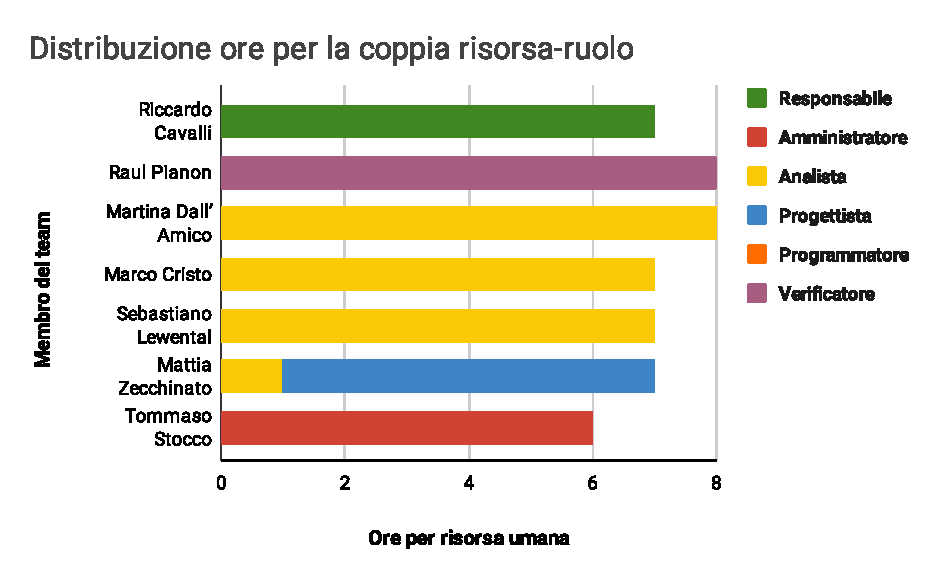
\includegraphics[width=0.90\textwidth]{assets/Consuntivo/Sprint-1/distribuzione_ore_risorsa_ruolo.pdf}
  \caption{Sprint 1 - Istogramma della distribuzione oraria per la coppia risorsa-ruolo}
\end{figure}

\begin{figure}[H]
  \centering
  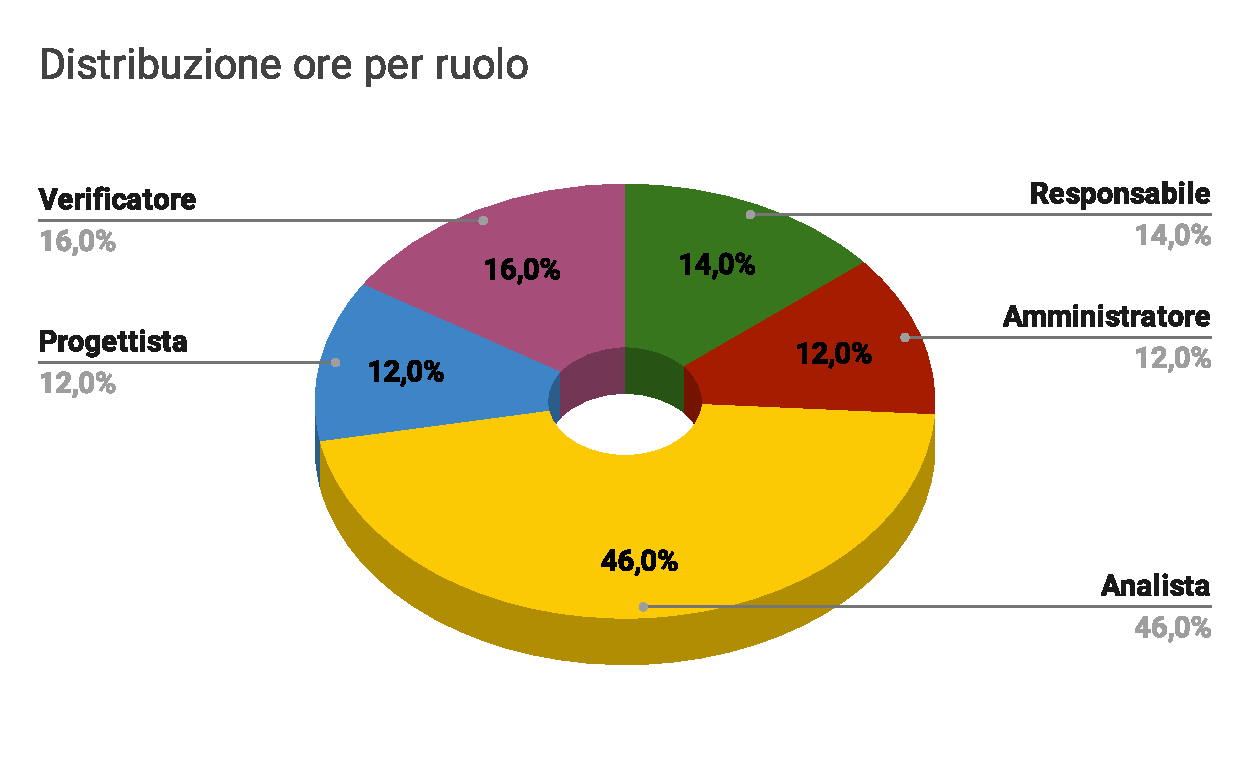
\includegraphics[width=0.90\textwidth]{assets/Consuntivo/Sprint-1/distribuzione_ore_ruolo.pdf}
  \caption{Sprint 1 - Areogramma della distribuzione oraria per ruolo}
\end{figure}

\begin{minipage}{\textwidth}
Di seguito è riportato il consuntivo economico del primo \glossario{sprint}:
\begin{table}[H]
\begin{adjustwidth}{-0.5cm}{-0.5cm}
  \centering
  \begin{tabular}{|P{2.9cm}|P{2.3cm}|P{2.5cm}|P{2.3cm}|>{\arraybackslash}P{2.5cm}|}
    \hline
    \multicolumn{5}{|c|}{\textbf{Consuntivo economico}} \\
    \hline
    \textbf{Ruolo} & \textbf{Ore per ruolo} & \textbf{Delta ore preventivo - consuntivo} & \textbf{Costo (in \texteuro)} & \textbf{Delta costo preventivo - consuntivo (in \texteuro)} \\
    \hline
    Responsabile & 7 & 0 & 210,00 & 0,00 \\
    \hline
    Amministratore & 6 & 0 & 120,00 & 0,00 \\
    \hline
    Analista & 23 & 4 & 575,00 & 100,00 \\
    \hline
    Progettista & 6 & 1 & 150,00 & 25,00 \\
    \hline
    Programmatore & 0 & 0 & 0,00 & 0,00 \\
    \hline
    Verificatore & 8 & 0 & 120,00 & 0,00 \\
    \hline
    \textbf{Totale} & \textbf{50} & 5 & \textbf{1.175,00} & 125,00 \\
    \hline
    \textbf{Restante} & 587 & / & 11.845,00 & / \\
    \hline
    \textbf{Sprint pregressi} & 0 & / & 0,00 & / \\
    \hline
  \end{tabular}
  \caption{Sprint 1 - Consuntivo economico}
\end{adjustwidth}
\end{table}
\end{minipage}

\begin{figure}[H]
  \centering
  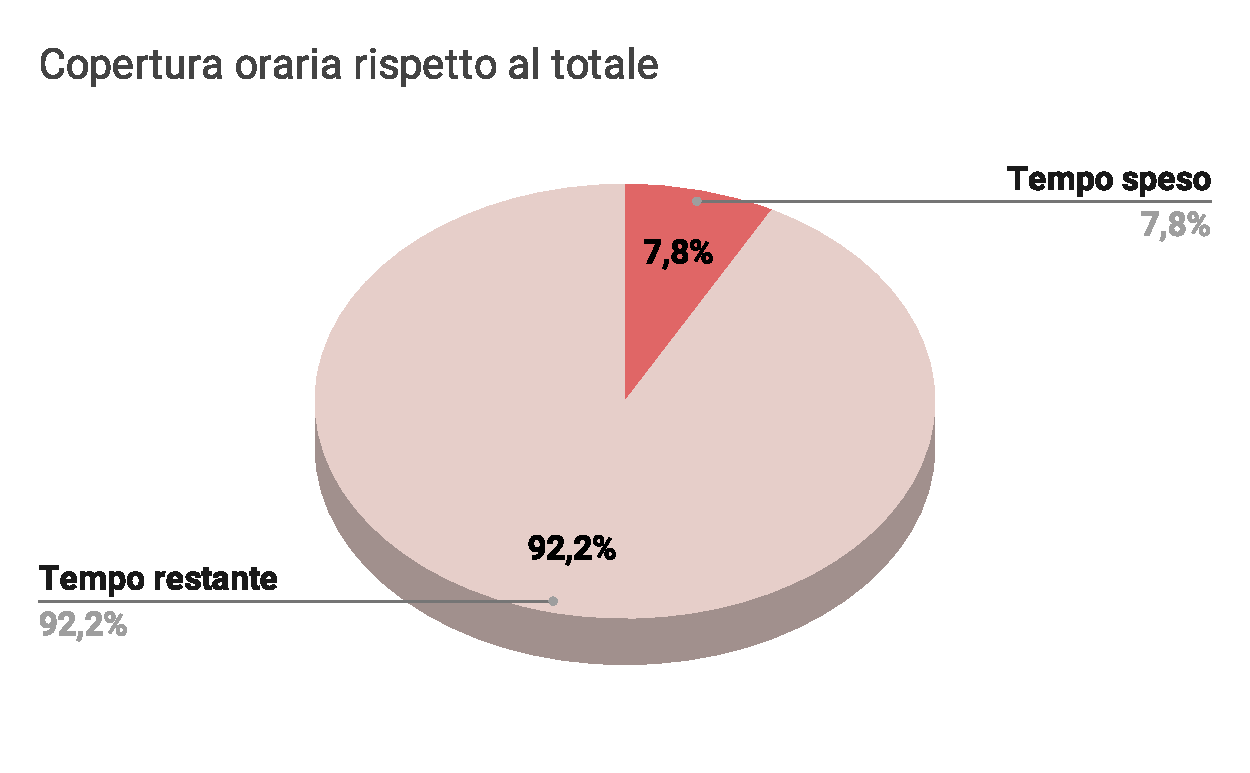
\includegraphics[width=0.90\textwidth]{assets/Consuntivo/Sprint-1/copertura_oraria.pdf}
  \caption{Sprint 1 - Areogramma del tempo speso (in ore) rispetto al totale}
\end{figure}

\begin{figure}[H]
  \centering
  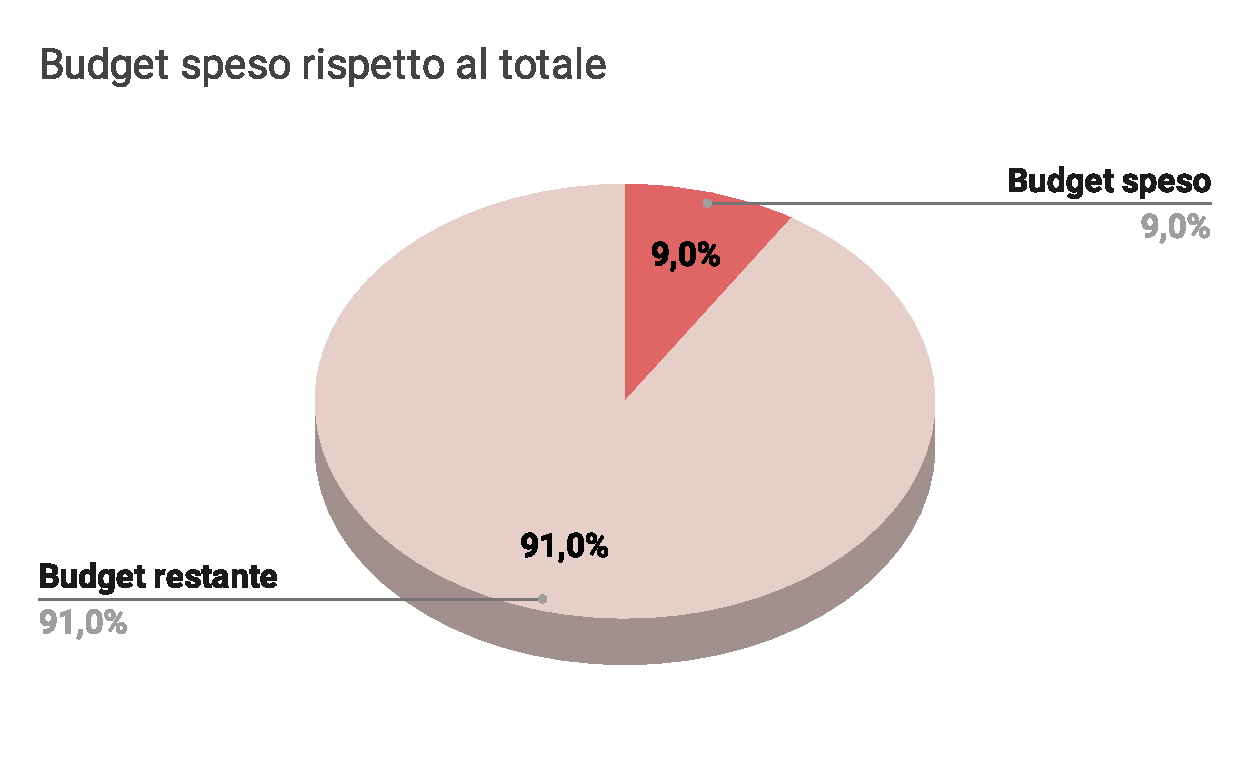
\includegraphics[width=0.90\textwidth]{assets/Consuntivo/Sprint-1/budget_speso.pdf}
  \caption{Sprint 1 - Areogramma del budget speso rispetto al totale}
\end{figure}


\begin{minipage}{\textwidth}
  Di seguito sono riportate le ore rimanenti per la coppia risorsa-ruolo:
  \begin{table}[H]
    \begin{tabularx}{\textwidth}{|c|*{6}{>{\centering}X|}c|}
      \hline
      \multicolumn{8}{|c|}{\textbf{Ore rimanenti per la coppia risorsa-ruolo}} \\
      \hline
      \textbf{Membro del team} & \textbf{Re} & \textbf{Am} & \textbf{An} & \textbf{Pt} & \textbf{Pr} & \textbf{Ve} & \textbf{Totale per persona} \\
      \hline
      Cavalli Riccardo & 2 & 8 & 9 & 23 & 22 & 20 & 84 \\
      \hline
      Pianon Raul & 9 & 8 & 9 & 23 & 22 & 12 & 83 \\
      \hline
      Dall'Amico Martina & 9 & 8 & 1 & 23 & 22 & 20 & 83 \\
      \hline
      Cristo Marco & 9 & 8 & 2 & 23 & 22 & 20 & 84 \\
      \hline
      Lewental Sebastiano & 9 & 8 & 2 & 23 & 22 & 20 & 84 \\
      \hline
      Zecchinato Mattia & 9 & 8 & 8 & 17 & 22 & 20 & 84 \\
      \hline
      Stocco Tommaso & 9 & 2 & 9 & 23 & 22 & 20 & 85 \\
      \hline
      \textbf{Totale per ruolo} & 56 & 50 & 40 & 155 & 154 & 132 & \textbf{587} \\
      \hline
    \end{tabularx}
    \caption{Sprint 1 - Ore rimanenti per la coppia risorsa-ruolo}
  \end{table}
\end{minipage}

\subsubsection{Revisione delle attività}

Nel corso del primo \glossario{sprint}, il team ha svolto le seguenti attività:
\begin{itemize}
  \item Stesura iniziale del \PdP;
  \item Scelta del modello di sviluppo;
  \item Pianificazione e preventivo del secondo \glossario{sprint};
  \item \AdR\ e definizione dei primi \glossario{casi d'uso};
  \item Individuazione degli \glossario{attori} coinvolti nel sistema e delle loro caratteristiche;
  \item Analisi dei rischi tecnologici e organizzativi;
  \item Composizione preliminare del \glossario{dizionario dati};
  \item Raccolta dei termini da inserire nel \Gls;
  \item Miglioramento del \WoW\ e automazione delle procedure con relativa stesura delle \NdP;
  \item Valutazione di eventuali alternative all'\glossario{Issue Tracking System} di \glossario{GitHub}.
\end{itemize}

\subsubsection{Retrospettiva}
\par Di seguito sono riportati i risultati del questionario di valutazione dello \glossario{sprint}, realizzato dal responsabile in carica per supportare la fase di \glossario{retrospettiva}:
\begin{itemize}
  \item Organizzazione dello \glossario{sprint} - Valutazione: 7,5;
  \item Conduzione dei meeting interni - Valutazione: 7,5;
  \item Conduzione dei meeting esterni - Valutazione: 8;
  \item Impegno e partecipazione dei singoli membri - Valutazione: 7;
  \item Non tutti i membri del team erano a conoscenza delle proprie mansioni;
  \item La numerosità delle riunioni è adeguata;
  \item Le riunioni sono state organizzate quasi sempre con il giusto preavviso;
  \item Da migliorare il rapporto ore spese/ore produttive.
\end{itemize}

\vspace{0.5\baselineskip}
\par A seguire le \textbf{analisi a posteriori} del primo \glossario{sprint}:
\begin{itemize}
  \item Le valutazioni raccolte dal team hanno evidenziato una pianificazione idonea ma non esaustiva. Di conseguenza, la transizione da un'attività a quella successiva non è sempre stata immediata, e ciò ha portato a delle fasi, seppur brevi, di stallo. Per tale motivo è stata registrata una discrepanza di 5 ore produttive rispetto a quanto definito nel preventivo;
  \item Inoltre, il gruppo ha ritenuto di aver sovrastimato il carico di lavoro per alcuni ruoli, in particolare l'analista e il progettista, a cui sono state assegnate 34 ore produttive totali. A posteriori, il team avrebbe preferito rimuovere una risorsa dal ruolo di analista, per assegnarla a mansioni impegnative come l'amministratore e il responsabile;
  \item Per via di una pianificazione non dettagliata, dell'inesperienza nell'\AdR\ e di una distribuzione non omogenea delle ore, il gruppo si è ritrovato a performare al di sotto delle aspettative in determinati ruoli. Tuttavia, la mancanza di uniformità nella ripartizione dei ruoli ha contruibuito alla creazione di micro-gruppi autonomi. Ciò ha favorito la condivisione delle conoscenze e il lavoro collaborativo, riducendo al minimo le perdite dal punto di vista dell'intensità di lavoro, che altrimenti sarebbero risultate pregiudizievoli;
  \item Il team ha riscontrato un feedback positivo per quanto riguarda l'organizzazione e la conduzione delle riunioni. Al contrario, sono stati rilevati come aspetti da migliorare la coesione interna e il rendimento delle singole risorse;
  \item Durante il primo \glossario{sprint}, il progettista ha lavorato a stretto contatto con il team di analisti. Perciò, la definizione del \glossario{dizionario dati} è passata in secondo piano rispetto al delineamento dell'architettura generale dell'applicazione. Questo ha comportato un aggiornamento della pianificazione, al fine di spostare la stesura del \glossario{dizionario dati} alla prossima iterazione;
  \item La redazione del verbale esterno del 3 aprile 2024 ha subito un ritardo per via dell'inesperienza del team nell'uso di \glossario{LaTeX}. Dal prossimo \glossario{sprint}, il gruppo si impegnerà ad aggiornare il template \glossario{LaTeX} (con l'aggiunta di parametri e comandi predefiniti) per velocizzare la stesura dei documenti. Inoltre, si è deciso di provare a rendere il contenuto dei verbali più asciutto e conciso. Ciò non significa però che si debba rinunciare a un resoconto dettagliato delle riunioni;
  \item Gli ostacoli principali dal punto organizzativo sono derivati dalla mancanza di una lista puntuale delle attività da svolgere. L'\glossario{Issue Tracking System} di \glossario{GitHub} non è stato sufficiente a garantire una corretta e completa gestione dei task. Per tale motivo, il team ha deciso di valutare l'adozione di \glossario{Jira Software} come \glossario{ITS}. Gli strumenti sviluppati da Atlassian, difatti, sembrano essere maggiormente orientati verso il modello \glossario{Agile}; inoltre, sono disponibili funzionalità come il calendario e la timeline che offrono una visione d'insieme del progetto e di eventuali ritardi;
  \item Nella prima metà dello \glossario{sprint}, la risorsa impiegata nel ruolo di verificatore ha ricevuto un carico di lavoro inferiore rispetto a quanto pianificato. Durante la riunione di \glossario{retrospettiva}, il team ha convenuto che, in futuro, le ore potenzialmente “dissipate” potrebbero essere utilizzate in modo produttivo se impiegate in un ruolo diverso.
\end{itemize}

\subsubsection{Aggiornamento pianificazione e preventivo}
\par Il team ha definito un piano d'azione per migliorare l'organizzazione e la produttività del prossimo \glossario{sprint}:
\begin{itemize}
  \item Definire una "To-Do List" più precisa;
  \item Organizzare riunioni brevi e mirate;
  \item Interazione più frequente tra il responsabile e il team di sviluppo;
  \item Pianificare lo studio delle tecnologie in maniera graduata;
  \item Verificare costantemente il progresso delle attività e la documentazione di progetto;
  \item Programmare un incontro in presenza con cadenza mensile;
  \item Sinergia tra ruoli con funzioni complementari;
  \item Sfruttare l'esperienza acquisita da chi ricopriva un ruolo in precedenza;
  \item Possibilità di assumere più ruoli durante uno \glossario{sprint};
  \item Distribuzione più omogenea delle ore tra i ruoli;
  \item Proseguire sulla strada dei micro-gruppi, suddividendo il lavoro in team più piccoli.
\end{itemize}

\paragraph*{Pianificazione futura:}
\par Come riportato nelle analisi a posteriori, il team ha posticipato la stesura del \glossario{dizionario dati} al secondo \glossario{sprint}. Inoltre, il team ha dovuto riconsiderare l’idea di partenza in merito allo studio delle tecnologie. Nella fase di candidatura, infatti, il gruppo aveva stabilito che, nell’arco del primo \glossario{sprint}, tutti i membri del gruppo avrebbero dovuto approfondire i linguaggi e le librerie proposte, specialmente \glossario{txtai}.

\vspace{0.5\baselineskip}
\par Questa pianificazione preliminare, tuttavia, non teneva conto delle attività di natura organizzativa, proprie del responsabile e dell’amministratore. Inoltre, la stesura della documentazione ha coperto la quasi totalità delle ore produttive del gruppo. Lo studio delle tecnologie è quindi stato spostato al prossimo periodo. In conclusione, la pianificazione del secondo \glossario{sprint} viene aggiornata con le seguenti attività:
\begin{itemize}
  \item Definizione del dizionario dati;
  \item Studio di \glossario{txtai} e creazione di programmi per testare le funzionalità della libreria.
\end{itemize}

\vspace{0.5\baselineskip}
\par Durante la riunione di \glossario{retrospettiva}, il team ha valutato anche la creazione di un file di configurazione da caricare nel \glossario{repository} documentale di \glossario{GitHub}. Attualmente, i documenti in formato PDF vengono generati in locale e caricati manualmente sul \glossario{repository} di vetrina. Tale operazione, però, è poco scalabile e vincolata alle prestazioni delle singole macchine. Viceversa, il file di configurazione consentirebbe di automatizzare la compilazione e la distribuzione dei documenti.


\paragraph*{Preventivo "a finire" (\sezione{sec:stima_temporale}):}
\par Per quanto riguarda il ruolo di analista, le ore non impiegate saranno reinvestite nello \glossario{sprint} a ridosso della \glossario{RTB}, al fine di rivedere i \glossario{casi d'uso} e apportare dei miglioramenti formali al documento di \AdR. L'ora produttiva di progettista, invece, sarà assegnata nel quarto \glossario{sprint}, per supportare l'attività di definizione dell'interfaccia grafica.

\vspace{0.5\baselineskip}
\par Durante la \glossario{retrospettiva} del primo periodo, il team ha evidenziato anche la necessità di velocizzare la fase di approvazione delle modifiche. Di conseguenza, si è deciso di aggiungere una risorsa al ruolo di verificatore nel prossimo \glossario{sprint}. Relativamente al calendario di massima del progetto, il gruppo non ha ritenuto di dover rielaborare la data stimata per la \glossario{RTB}. Nei prossimi \glossario{sprint}, invece, verrà valutata la possibilità di designare alcune ore di progettista al ruolo di amministratore.

\paragraph*{Gestione dei rischi (\sezione{sec:analisi_rischi}):}
\par Durante il primo \glossario{sprint}, il team ha riscontrato l'affioramento di un rischio inatteso:
\begin{itemize}
  \item \textbf{Risorse disponibili ma non impiegate:} durante il primo \glossario{sprint}, il team non ha elaborato un numero sufficiente di documenti affinchè il verificatore potesse mantenere un'intensità di lavoro elevata. Di conseguenza, la media produttiva giornaliera della risorsa impiegata in tale ruolo non è rimasta costante. Dato il cospicuo numero di attività da svolgere, il team ritiene che la staticità dei ruoli sia inconciliabile con la metodologia scelta. Nella sezione di analisi dei rischi è stato quindi aggiunto un ulteriore rischio organizzativo. Secondo quanto stimato dal gruppo, la probabilità che il rischio si verifichi è alta, mentre il grado di criticità è medio. A partire dal prossimo periodo, il team si pone come obiettivo rendere più dinamica l'assegnazione delle attività.
\end{itemize}

\vspace{0.5\baselineskip}
\par Nel corso dello \glossario{sprint}, alcune contromisure si sono rivelate insufficienti per mitigare i rischi individuati in fase di pianificazione; perciò il gruppo ha deciso di aggiornare l'analisi dei rischi. In particolare, sono stati rivalutati i seguenti rischi:
\begin{itemize}
  \item \textbf{Scarso know-how tecnologico:} il gruppo ha aggiornato la probabilità di occorrenza del rischio legato all'uso di tecnologie, spostandola da "media" ad "alta". Dal prossimo \glossario{sprint}, infatti, si prevede di introdurre, oltre a \glossario{LaTeX} e \glossario{Docker}, altri strumenti come \glossario{Jira}, \glossario{txtai}, \glossario{YAML}, \glossario{JSON} e \glossario{Python}. Le misure precedentemente adottate si sono rivelate incomplete poiché non consideravano la possibilità di lavorare in coppia per risolvere un problema. Inoltre, il team ritiene di non dover sospendere il lavoro per apprendere nuove tecnologie, assegnando piuttosto lo studio a un gruppo ristretto di risorse. Tale gruppo terrà poi un workshop per condividere le conoscenze. In aggiunta, il team ha migliorato le strategie di rilevamento del rischio tecnologico, introducendo ad esempio la \glossario{continuous integration}. Le modifiche complete sono visibili nella sezione di analisi dei rischi;
  \item \textbf{Rischio legato all'inesperienza:} tale rischio, considerato troppo vago e dispersivo, è stato rinominato in "Sottostima delle risorse necessarie per un'attività". Per migliorare la gestione del rischio, il team ha definito con maggior rigore il processo di suddivisione dei task in sotto-attività. Le misure di mitigazione, documentate nella sezione di analisi dei rischi, hanno l'obiettivo di ridurre gli impatti negativi sui task successivi.
\end{itemize}




\subsubsection{Sprint 2: da 2024-04-22 a 2024-05-06}
\begin{minipage}{\textwidth}
Di seguito è riportata la distribuzione delle ore per ciascun membro del team, accumulate in totali per persona e per ruolo:
\begin{table}[H]
  \begin{tabularx}{\textwidth}{|c|*{6}{>{\centering}X|}c|}
    \hline
    \multicolumn{8}{|c|}{\textbf{Preventivo orario}} \\
    \hline
    \textbf{Membro del team} & \textbf{Re} & \textbf{Am} & \textbf{An} & \textbf{Pt} & \textbf{Pr} & \textbf{Ve} & \textbf{Totale per persona} \\
    \hline
    Riccardo Cavalli & 0 & 7 & 0 & 0 & 0 & 0 & 7 \\
    \hline
    Raul Pianon & 7 & 0 & 0 & 0 & 0 & 0 & 7 \\
    \hline
    Martina Dall'Amico & 0 & 0 & 0 & 0 & 0 & 6 & 6 \\
    \hline
    Marco Cristo & 0 & 0 & 0 & 0 & 8 & 0 & 8 \\
    \hline
    Sebastiano Lewental & 0 & 0 & 0 & 7 & 0 & 0 & 7 \\
    \hline
    Mattia Zecchinato & 0 & 0 & 0 & 0 & 0 & 6 & 6 \\
    \hline
    Tommaso Stocco & 0 & 0 & 7 & 0 & 0 & 0 & 7 \\
    \hline
    \textbf{Totale per ruolo} & 7 & 7 & 7 & 7 & 8 & 12 & \textbf{48} \\
    \hline
  \end{tabularx}
  \caption{Sprint 2 - Preventivo orario}
\end{table}
\end{minipage}

\begin{figure}[H]
  \centering
  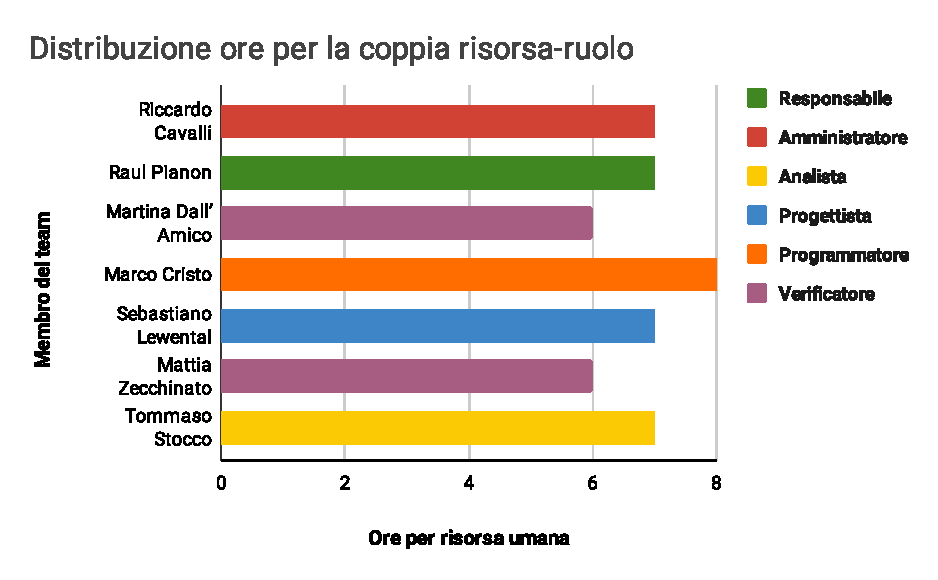
\includegraphics[width=0.90\textwidth]{assets/Preventivo/Sprint-2/distribuzione_ore_risorsa_ruolo.pdf}
  \caption{Sprint 2 - Istogramma della distribuzione oraria per la coppia risorsa-ruolo}
\end{figure}

\begin{figure}[H]
  \centering
  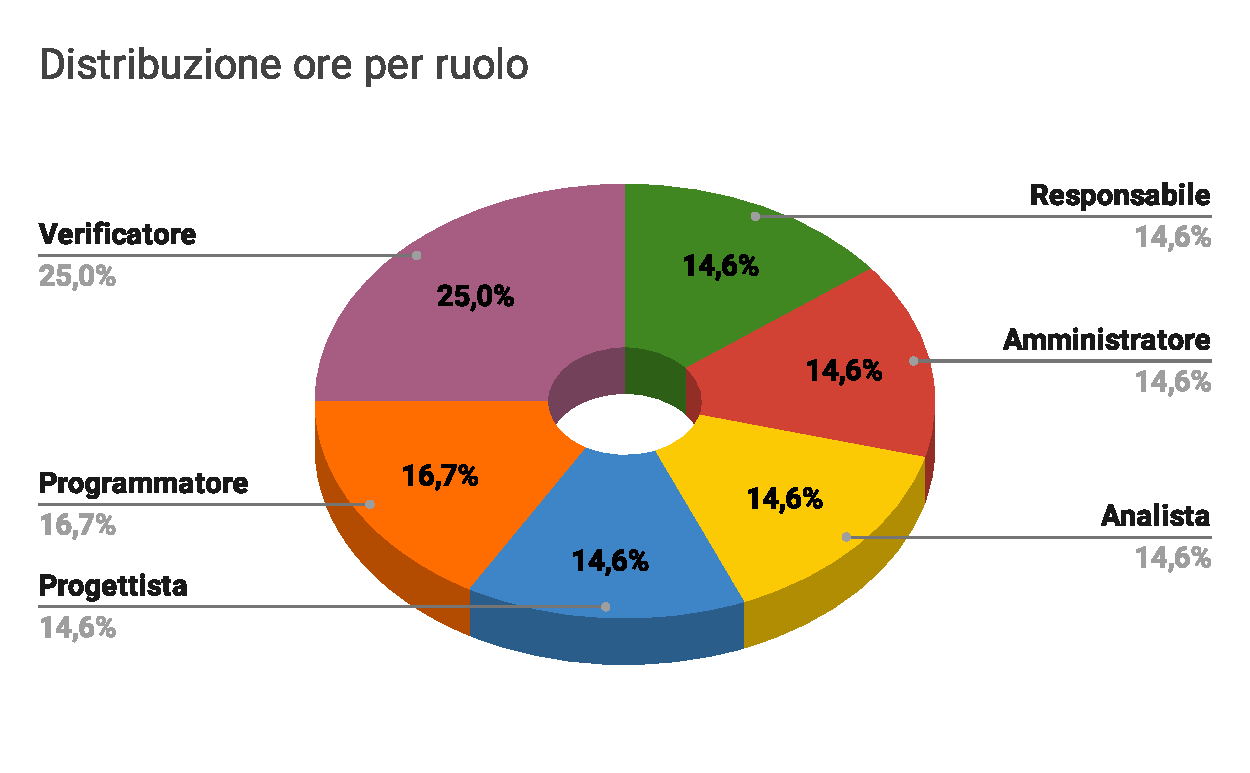
\includegraphics[width=0.90\textwidth]{assets/Preventivo/Sprint-2/distribuzione_ore_ruolo.pdf}
  \caption{Sprint 2 - Areogramma della distribuzione oraria per ruolo}
\end{figure}

\begin{minipage}{\textwidth}
Di seguito è riportato il preventivo economico del secondo \glossario{sprint}:
\begin{table}[H]
  \centering
  \begin{tabular}{|c|c|c|}
    \hline
    \multicolumn{3}{|c|}{\textbf{Preventivo economico}} \\
    \hline
    \textbf{Ruolo} & \textbf{Ore per ruolo} & \textbf{Costo (in \texteuro)} \\
    \hline
    Responsabile & 7 & 210,00 \\
    \hline
    Amministratore & 7 & 140,00 \\
    \hline
    Analista & 7 & 175,00 \\
    \hline
    Progettista & 7 & 175,00 \\
    \hline
    Programmatore & 8 & 120,00 \\
    \hline
    Verificatore & 12 & 180,00 \\
    \hline
    \textbf{Totale} & 48 & \textbf{1.000,00} \\
    \hline
  \end{tabular}
  \caption{Sprint 2 - Preventivo economico}
\end{table}
\end{minipage}
\subsection{Terzo sprint}

\begin{minipage}{\textwidth}
  Di seguito è riportata la distribuzione delle ore per ciascun membro del team, accumulate in totali per persona e per ruolo:
  \begin{table}[H]
    \begin{tabularx}{\textwidth}{|c|*{6}{>{\centering}X|}c|}
      \hline
      \multicolumn{8}{|c|}{\textbf{Consuntivo orario}} \\
      \hline
      \textbf{Membro del team} & \textbf{Re} & \textbf{Am} & \textbf{An} & \textbf{Pt} & \textbf{Pr} & \textbf{Ve} & \textbf{Totale per persona} \\
      \hline
      Cavalli Riccardo & 1 & 2 & 0 & 6 & 2 & 0 & 11 \\
      \hline
      Pianon Raul & 0 & 0 & 0 & 0 & 8 & 0 & 8 \\
      \hline
      Dall'Amico Martina & 0 & 8 & 0 & 0 & 0 & 0 & 8 \\ 
      \hline
      Cristo Marco & 0 & 0 & 0 & 0 & 5 & 2 & 7 \\ 
      \hline
      Lewental Sebastiano & 0 & 0 & 0 & 3 & 2 & 3 & 8 \\ 
      \hline
      Zecchinato Mattia & 0 & 1 & 5 & 0 & 0 & 0 & 6 \\ 
      \hline
      Stocco Tommaso & 4 & 0 & 0 & 0 & 0 & 2 & 6 \\ 
      \hline
      \textbf{Totale ore per ruolo} & 5 & 11 & 5 & 9 & 17 & 7 & \textbf{54} \\
      \hline
    \end{tabularx}
    \caption{Sprint 3 - Consuntivo orario}
  \end{table}
  \end{minipage}
  
  \begin{figure}[H]
    \centering
    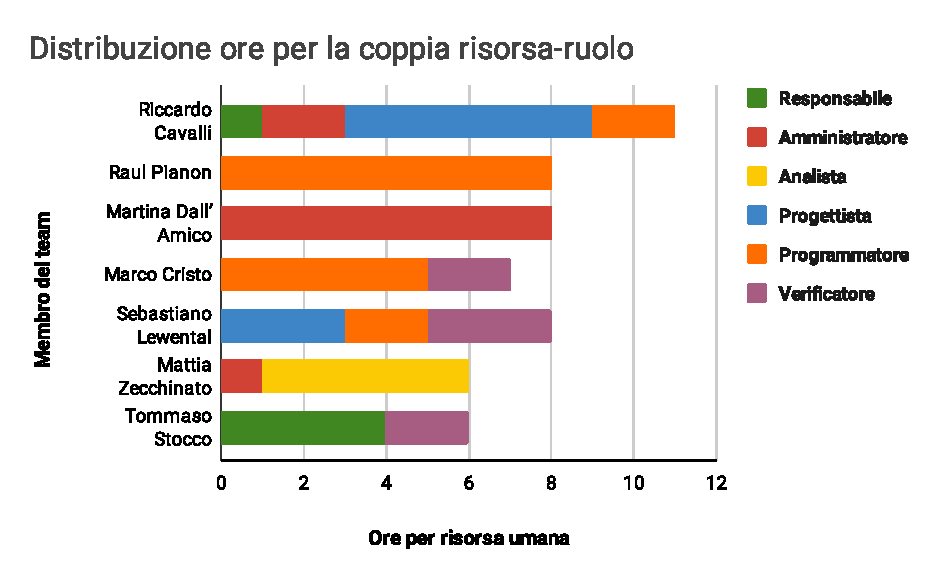
\includegraphics[width=0.90\textwidth]{assets/Consuntivo/Sprint-3/distribuzione_ore_risorsa_ruolo.pdf}
    \caption{Sprint 3 - Istogramma della distribuzione oraria per la coppia risorsa-ruolo}
  \end{figure}
  
  \begin{figure}[H]
    \centering
    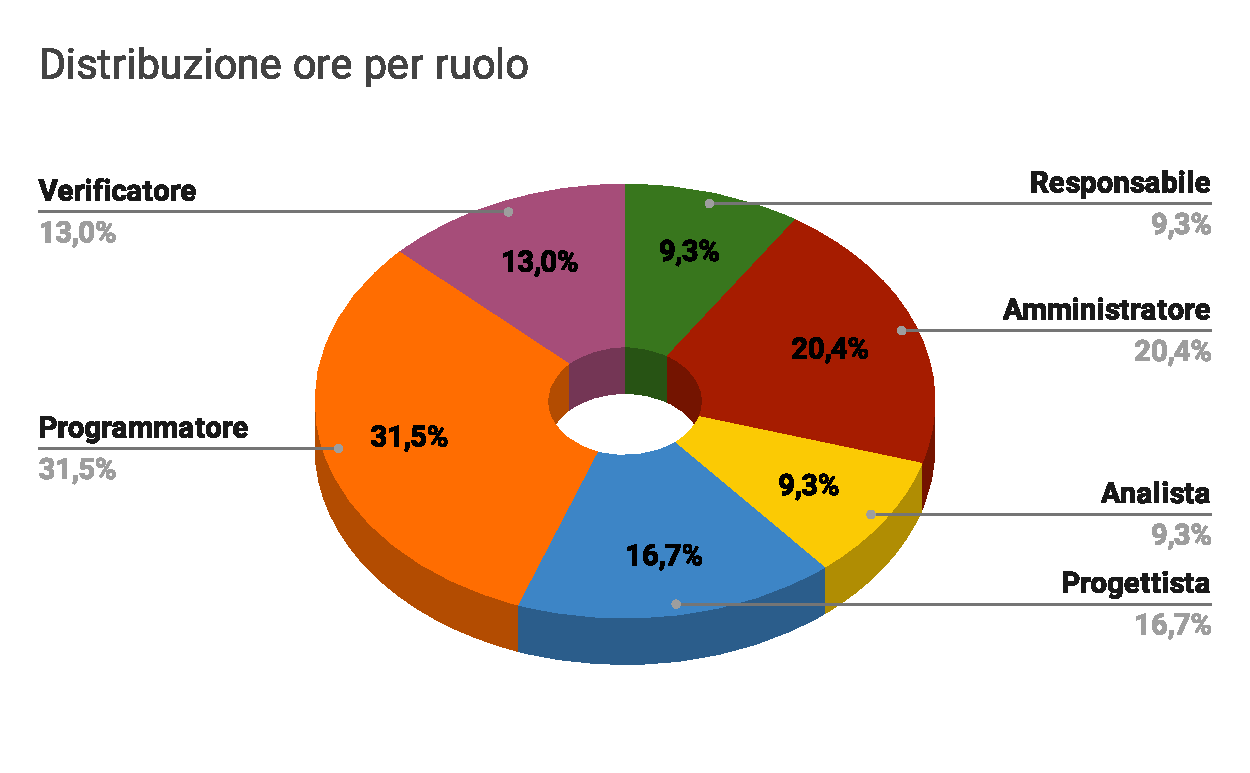
\includegraphics[width=0.90\textwidth]{assets/Consuntivo/Sprint-3/distribuzione_ore_ruolo.pdf}
    \caption{Sprint 3 - Areogramma della distribuzione oraria per ruolo}
  \end{figure}
  
  \begin{minipage}{\textwidth}
  Di seguito è riportato il consuntivo economico del terzo \glossario{sprint}:
  \begin{table}[H]
  \begin{adjustwidth}{-0.5cm}{-0.5cm}
    \centering
    \begin{tabular}{|P{2.9cm}|P{2.3cm}|P{2.5cm}|P{2.3cm}|>{\arraybackslash}P{2.5cm}|}
      \hline
      \multicolumn{5}{|c|}{\textbf{Consuntivo economico}} \\
      \hline
      \textbf{Ruolo} & \textbf{Ore per ruolo} & \textbf{Delta ore preventivo - consuntivo} & \textbf{Costo (in \texteuro)} & \textbf{Delta costo preventivo - consuntivo (in \texteuro)} \\
      \hline
      Responsabile & 5 & +1 & 150,00 & +30,00 \\ 
      \hline
      Amministratore & 11 & +1 & 220,00 & +20,00 \\ 
      \hline
      Analista & 5 & -1 & 125,00 & -25,00 \\ 
      \hline
      Progettista & 9 & -3 & 225,00 & -75,00 \\ 
      \hline
      Programmatore & 17 & -1 & 255,00 & -15,00 \\ 
      \hline
      Verificatore & 7 & 0 & 105,00 & 0,00 \\ 
      \hline
      \textbf{Totale} & \textbf{54} & -3 & \textbf{1.080,00} & -65,00 \\ 
      \hline
      \textbf{Restante} & 488 & / & 9.790,00 & / \\ 
      \hline
      \textbf{Sprint pregressi} & 95 & / & 2.150,00 & / \\ 
      \hline
    \end{tabular}
    \caption{Sprint 3 - Consuntivo economico}
  \end{adjustwidth}
  \end{table}
  \end{minipage}
  
  \begin{figure}[H]
    \centering
    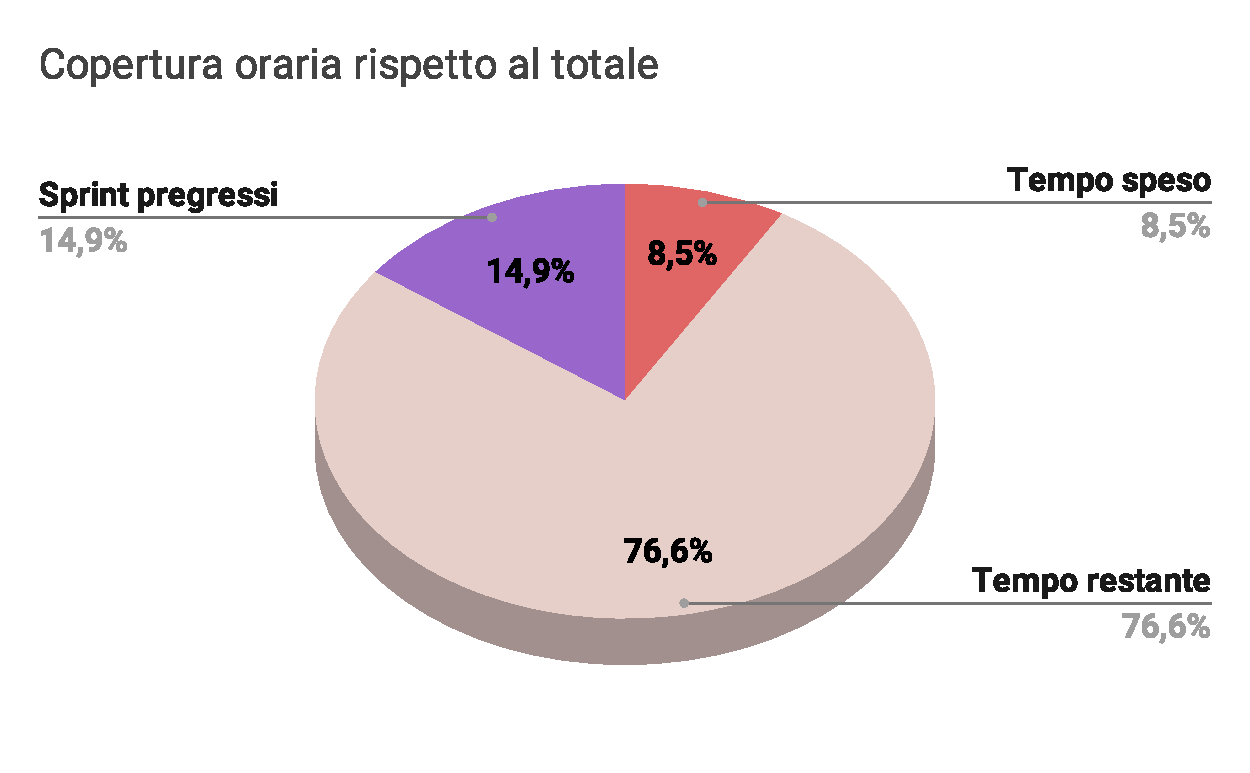
\includegraphics[width=0.90\textwidth]{assets/Consuntivo/Sprint-3/copertura_oraria.pdf}
    \caption{Sprint 3 - Areogramma del tempo speso (in ore) rispetto al totale}
  \end{figure}
  
  \begin{figure}[H]
    \centering
    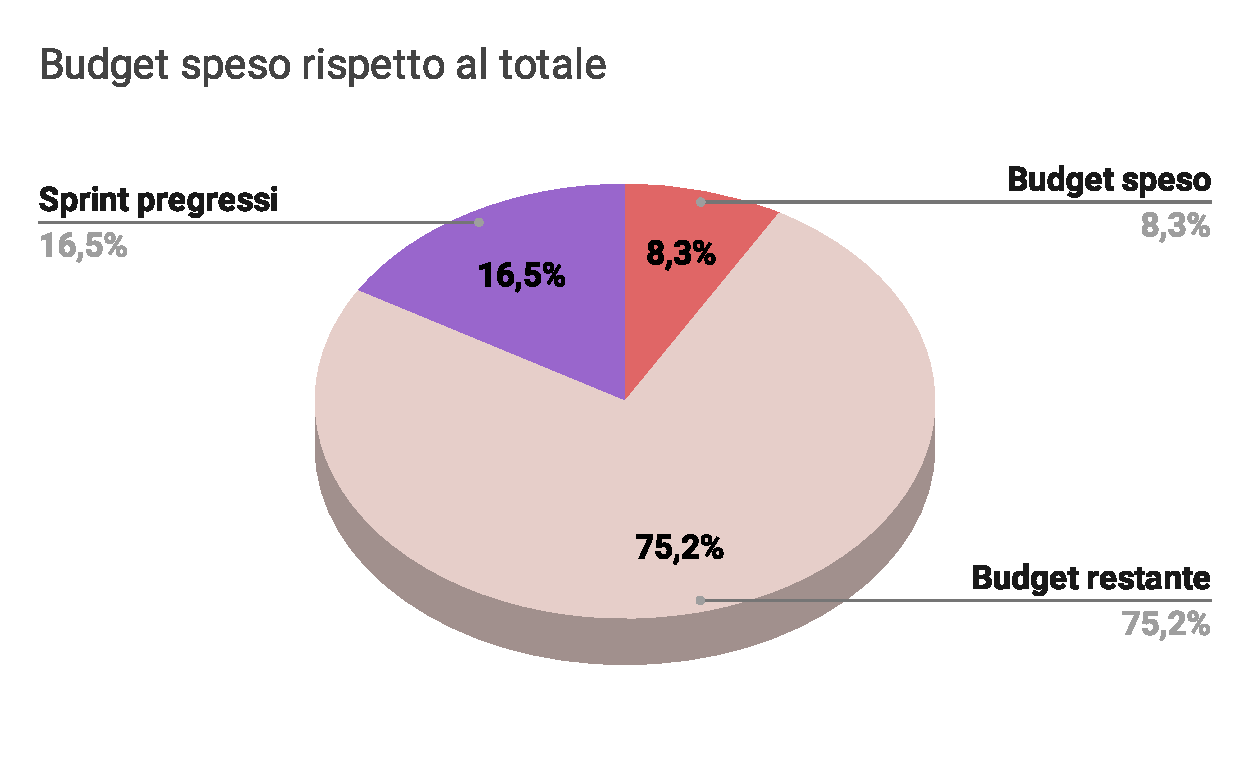
\includegraphics[width=0.90\textwidth]{assets/Consuntivo/Sprint-3/budget_speso.pdf}
    \caption{Sprint 3 - Areogramma del budget speso rispetto al totale}
  \end{figure}
  
  \begin{minipage}{\textwidth}
    Di seguito sono riportate le ore rimanenti per la coppia risorsa-ruolo:
    \begin{table}[H]
      \begin{tabularx}{\textwidth}{|c|*{6}{>{\centering}X|}c|}
        \hline
        \multicolumn{8}{|c|}{\textbf{Ore rimanenti per la coppia risorsa-ruolo}} \\
        \hline
        \textbf{Membro del team} & \textbf{Re} & \textbf{Am} & \textbf{An} & \textbf{Pt} & \textbf{Pr} & \textbf{Ve} & \textbf{Totale per persona} \\
        \hline
        Cavalli Riccardo & 0 & 0 & 9 & 17 & 20 & 20 & 66 \\ 
        \hline
        Pianon Raul & 2 & 8 & 9 & 23 & 14 & 12 & 68 \\ 
        \hline
        Dall'Amico Martina & 9 & 0 & 1 & 23 & 22 & 15 & 70 \\ 
        \hline
        Cristo Marco & 9 & 8 & 2 & 20 & 12 & 18 & 69 \\ 
        \hline
        Lewental Sebastiano & 9 & 8 & 2 & 14 & 20 & 17 & 70 \\ 
        \hline
        Zecchinato Mattia & 9 & 7 & 3 & 17 & 22 & 14 & 72 \\ 
        \hline
        Stocco Tommaso & 5 & 2 & 3 & 23 & 22 & 18 & 73 \\ 
        \hline
        \textbf{Totale ore per ruolo} & 43 & 33 & 29 & 137 & 132 & 114 & \textbf{488} \\ 
        \hline
      \end{tabularx}
      \caption{Sprint 3 - Ore rimanenti per la coppia risorsa-ruolo}
    \end{table}
  \end{minipage}

\subsubsection{Revisione delle attività}

Nell'arco del terzo \glossario{sprint}, il team ha svolto le seguenti attività:
\begin{itemize}
    \item Stesura verbali interni ed esterni;
    \item Push e pull dell'immagine \glossario{Docker} su \glossario{GitHub Container Registry};
    \item Aggiornamento delle \NdP\ con le modalità di integrazione Jira - Github;
    \item Riformulazione del dizionario dati (chiavi primarie, chiavi esterne e sinonimi);
    \item Creazione della prima bozza dell'interfaccia grafica;
    \item Studio del framework \glossario{Streamlit} e inizio sviluppo della web app;
    \item Definizione di un indice aggiuntivo per ricavare le informazioni delle tabelle pertinenti alla richiesta dell'utente;	
    \item Modifica struttura del PdP\ e approfondimento della sezione relativa al consuntivo;
    \item Selezione e descrizione delle metriche M1, M2, M3, M4;
    \item Scelta dei range di tolleranza per le metriche M1, M2, M3, M4;
    \item Benchmark iniziale dei modelli;
    \item Unificazione dei differenti metodi di estrazione del \glossario{dizionario dati} in un modulo unico;
    \item Stesura delle sezioni incomplete nel documento di \AdR;
    \item Espansione dei casi d'uso e rifinitura delle definizioni dei requisiti e delle fonti;
    \item Approfondimento del funzionamento di \glossario{txtai};
    \item Creazione di un dizionario dati in italiano per testare il modello sentence-BERTino di efederici;
    \item Prova di traduzione della richiesta utente;
    \item Costruzione della query SQL per la ricerca semantica;
    \item Aggiunta dei sinonimi delle tabelle e delle colonne nell'\glossario{indice};
    \item Miglioramento della ricerca semantica tramite la media pesata dei punteggi;
    \item Definizione di un workflow su GitHub Actions per il repository di sviluppo;
    \item Preventivo dello sprint 4;
    \item Elaborazione di una presentazione sul framework Streamlit;
    \item Configurazione di \glossario{Flask} e \glossario{Django} come framework back-end alternativi.
\end{itemize}

\subsubsection{Retrospettiva}

\par Di seguito sono riportati i risultati del questionario di valutazione dello \glossario{sprint}:
\begin{itemize}
  \item Organizzazione dello \glossario{sprint}\ - Valutazione: 8;
  \item Conduzione dei meeting interni - Valutazione: 8;
  \item Conduzione dei meeting esterni - Valutazione: 7,5;
  \item Impegno e partecipazione dei singoli membri - Valutazione: 8;
  \item La quasi totalità dei membri del team era a conoscenza delle proprie mansioni;
  \item La numerosità delle riunioni è adeguata, anche se il team preferirebbe organizzare più incontri informali tra membri che ricoprono ruoli affini;
  \item Le riunioni sono state organizzate quasi sempre con il giusto preavviso;
  \item Il rapporto ore spese/ore produttive è discreto, ma può essere ancora migliorato;
  \item La produttività generale deve essere incrementata;
  \item Alcuni membri del team ritengono sia necessario un maggior controllo sulle attività da parte del responsabile.
\end{itemize}

\vspace{0.5\baselineskip}
\par A seguire le \textbf{analisi a posteriori} del terzo \glossario{sprint}:
\begin{itemize}
  \item Nonostante quanto emerso dal consuntivo orario, dove l'assegnazione temporale per ruolo è risultata sbilanciata a favore dei ruoli più tecnici (analista, progettista, programmatore) rispetto a quelli amministrativi (amministratore, responsabile), il team ha ritenuto opportuno non allocare ulteriori risorse a questi ultimi per concentrare gli sforzi sullo sviluppo del PoC;
  \item In seguito alle considerazioni del team riguardo la necessità di una maggiore supervisione da parte del responsabile, quest'ultimo dovrà impegnarsi, a partire dalla prossima iterazione, a stabilire degli intervalli di tempo sufficientemente brevi alla fine dei quali verificare lo stato di avanzamento delle attività;
  \item La conduzione delle riunioni esterne ha evidenziato l'inesperienza del team nel rapporto con la \glossario{Proponente}, che assume a tutti gli effetti il ruolo di cliente, le cui conoscenze tecniche sono spesso asimmetriche rispetto a quelle dei fornitori. La discussione dei dettagli implementativi è un processo interno al gruppo e, pertanto, non deve coinvolgere il cliente. In futuro sarà quindi opportuno mantenere la discussione a un livello più alto, concentrandosi sul "cosa" piuttosto che sul "come";
  \item Malgrado le difficoltà nell'individuare gli standard per la gestione dei servizi IT, i membri con il ruolo di amministratore sono stati in grado di reperire sufficiente documentazione, seppur meno recente, per un'adeguata stesura delle metriche di qualità e la loro categorizzazione;
  \item Sebbene \glossario{Streamlit} abbia dei limiti dal punto di vista del design, il team ha deciso di investire un numero cospicuo di risorse nella progettazione dell'interfaccia grafica. In questo modo, qualora il gruppo dovesse scegliere di cambiare \glossario{framework}, la transizione risulterebbe meno gravosa.
\end{itemize}

\subsubsection{Aggiornamento pianificazione e preventivo}
\par Il team ha definito un piano d'azione per migliorare l'organizzazione e la produttività del prossimo \glossario{sprint}:
\begin{itemize}
  \item Ridurre la rendicontazione produttiva di ore spese per studi che non avanzano concretamente lo stato del progetto;
  \item Definire delle \glossario{metriche di qualità} da applicare nel corso dello sviluppo dell'applicativo e non in retrospettiva;
  \item Impostare dei test per valutare la correttezza del \glossario{prompt};
  \item Aumentare l'interazione tra analisti, progettisti e programmatori;
  \item Definire una vista dei log per analisi più puntuali dei risultati;
\end{itemize}

\paragraph*{Pianificazione futura:}
Data l'assenza di una suite di test automatici, il \glossario{benchmark} dei modelli di \glossario{sentence similarity} ha richiesto uno sforzo maggiore in termini di tempo e non ha prodotto risultati sufficientemente attendibili. Di conseguenza, il team ha aggiornato la pianificazione del prossimo \glossario{sprint}, fissando come task ad alta priorità la definizione dei test di unità. Mediante l'esecuzione automatica di una batteria di test, il gruppo ritiene di poter verificare con maggior rigore l'affidabilità dei modelli di AI scelti. Come definito nella \glossario{retrospettiva}, il team non ha ancora finalizzato la scelta delle tecnologie, in quanto lo sviluppo degli scenari critici verrà ultimato nel prossimo \glossario{sprint}. Pertanto, il gruppo ha stabilito di proseguire l'analisi di framework alternativi anche nel prossimo periodo, al termine del quale verrà presa una decisione definitiva. La \glossario{dockerizzazione} dell'ambiente di sviluppo, invece, è stata pianificata per lo \glossario{sprint} 5. Le dipendenze del progetto verranno infatti delineate nell'arco della prossima iterazione.
\par Per quanto riguarda le metriche di qualità, il team ha fissato i seguenti obiettivi:
\begin{itemize}
  \item Individuazione delle metriche più significative;
  \item Identificazione di strumenti per automatizzare il calcolo delle metriche.
\end{itemize}
\par Dopo aver preso in considerazione un ampio insieme di indicatori, il gruppo ritiene infatti necessario operare una scrematura delle metriche individuate.

\paragraph*{Preventivo "a finire" (\sezione{sec:stima_temporale}):}
Il consuntivo del terzo \glossario{sprint} ha evidenziato una discrepanza di tre ore produttive rispetto a quanto preventivato. Questo perché la maggior parte del tempo è stata impiegata nello studio e nella valutazione delle tecnologie per il \glossario{PoC}. Nonostante i programmatori abbiano iniziato lo sviluppo del prototipo con \glossario{Streamlit}, il team ha ritenuto opportuno esaminare \glossario{framework} alternativi come \glossario{Django}, \glossario{Vue.js} e \glossario{Next.js}. Inoltre, l’uso delle funzionalità avanzate di \glossario{txtai} e la progettazione della bozza dell’interfaccia grafica hanno richiesto una fase di studio non indifferente. Per tale motivo, il gruppo ha deciso di rivedere il calendario di massima del progetto. Nel prossimo sprint, infatti, il team si focalizzerà sullo sviluppo dei \glossario{casi d’uso} all’interno dell’applicazione. Qualora la risposta di \glossario{Streamlit} dovesse risultare negativa (in termini di flessibilità, prestazioni e personalizzazione), il gruppo dovrebbe optare per due nuovi framework (back-end e front-end). Dunque, il team ha ridefinito la finestra temporale per la revisione \glossario{RTB} come segue:
\begin{itemize}
  \item Data di inizio: 2024-06-03;
  \item Scadenza: 2024-06-14.
\end{itemize}

\paragraph*{Gestione dei rischi (\sezione{sec:analisi_rischi}):}
\par Nel corso del terzo \glossario{sprint}, il team ha riscontrato l'affioramento di un rischio inatteso:
\begin{itemize}
  \item \textbf{Rischi relativi ad esigenze personali:} Nonostante il largo anticipo della comunicazione, l'impossibilità di uno dei membri del team di svolgere i propri incarichi, ha comportato la ridistribuzione di questi ultimi tra i restanti membri dai ruoli affini. 
  Questa forma di mitigazione ha avuto un successo parziale: lo sviluppo dell'\AdR\, seppur non interrotto, ha subito rallentamenti.
  Di conseguenza, il team ha ritenuto opportuno l'ampiamento della \sezione{sec:analisi_rischi} con una sottosezione relativa ai rischi di natura personale, rifinendo l'approccio adottato al netto dei rallentamenti come misura di mitigazione finale.
\end{itemize}

\vspace{0.5\baselineskip}
\par Durante il terzo \glossario{sprint}, alcune contromisure si sono rivelate utili a mitigare i rischi individuati in fase di pianificazione. In particolare:
\begin{itemize}
  \item \textbf{Rischi relativi alla collaborazione:} Durante il terzo \glossario{sprint}, il team ha ritenuto opportuno raccogliere, confrontare e infine integrare le opinioni (talvolta discordanti) di ciascun membro riguardo le regole interne, al fine di garantire una collaborazione proficua e continua tra i membri;
  \item \textbf{Malfunzionamenti software}: La configurazione di \glossario{Docker} e dell'ambiente di sviluppo ha causato malfunzionamenti software. Tuttavia, l'organizzazione tempestiva di incontri su Discord tra i membri interessati e i componenti con più esperienza ha prontamente risolto tali problematiche;
  \item \textbf{Rischi relativi alla rotazione dei ruoli}: Durante i primi \glossario{sprint}, diversi membri del gruppo hanno mantenuto le stesse mansioni per l'intera durata dell'iterazione, non riuscendo ad approfondire le proprie conoscenze al di fuori del ruolo assegnato. Questo ha provocato incertezze durante la rotazione dei ruoli da uno sprint all'altro. Le riunioni frequenti e il sostegno reciproco durante la transizione dei ruoli sono stati fondamentali per compensare la mancanza di esperienza.
\end{itemize}

\subsubsection{Sprint 4: da 2024-05-22 a 2024-06-03}
\begin{minipage}{\textwidth}
Di seguito è riportata la distribuzione delle ore per ciascun membro del team, accumulate in totali per persona e per ruolo:
\begin{table}[H]
  \begin{tabularx}{\textwidth}{|c|*{6}{>{\centering}X|}c|}
    \hline
    \multicolumn{8}{|c|}{\textbf{Preventivo orario}} \\
    \hline
    \textbf{Membro del team} & \textbf{Re} & \textbf{Am} & \textbf{An} & \textbf{Pt} & \textbf{Pr} & \textbf{Ve} & \textbf{Totale per persona} \\
    \hline
    Cavalli Riccardo & 0 & 0 & 0 & 0 & 3 & 6 & 9 \\
    \hline
    Pianon Raul & 0 & 0 & 6 & 0 & 0 & 2 & 8 \\
    \hline
    Dall'Amico Martina & 0 & 0 & 0 & 6 & 2 & 0 & 8 \\
    \hline
    Cristo Marco & 6 & 0 & 0 & 0 & 0 & 2 & 8 \\
    \hline
    Lewental Sebastiano & 0 & 7 & 0 & 0 & 0 & 0 & 7 \\
    \hline
    Zecchinato Mattia & 0 & 3 & 0 & 3 & 0 & 0 & 6 \\
    \hline
    Stocco Tommaso & 0 & 0 & 0 & 0 & 8 & 0 & 8 \\
    \hline
    \textbf{Totale per ruolo} & 6 & 10 & 6 & 9 & 13 & 10 & \textbf{54} \\
    \hline
  \end{tabularx}
  \caption{Sprint 4 - Preventivo orario}
\end{table}
\end{minipage}

\begin{figure}[H]
  \centering
  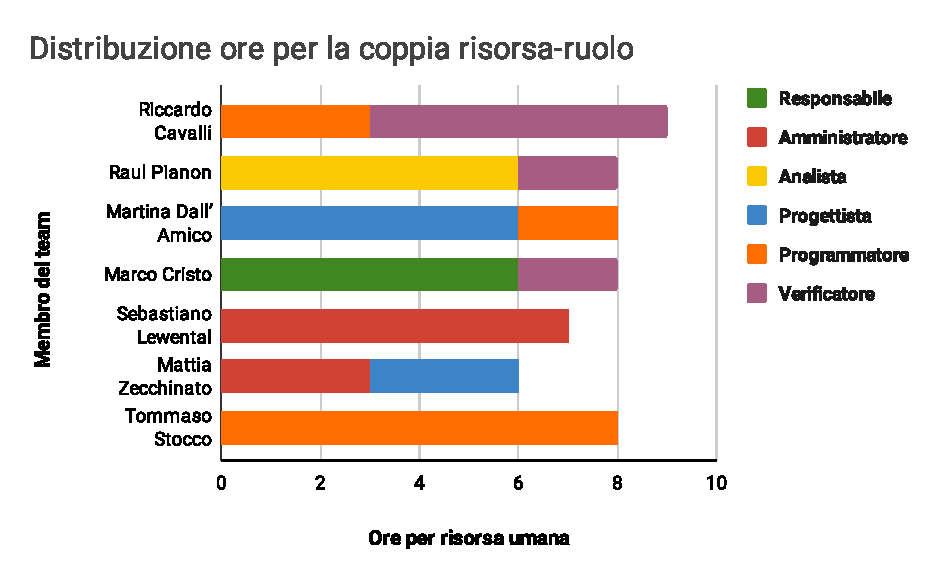
\includegraphics[width=0.90\textwidth]{assets/Preventivo/Sprint-4/distribuzione_ore_risorsa_ruolo.pdf}
  \caption{Sprint 4 - Istogramma della distribuzione oraria per la coppia risorsa-ruolo}
\end{figure}

\begin{figure}[H]
  \centering
  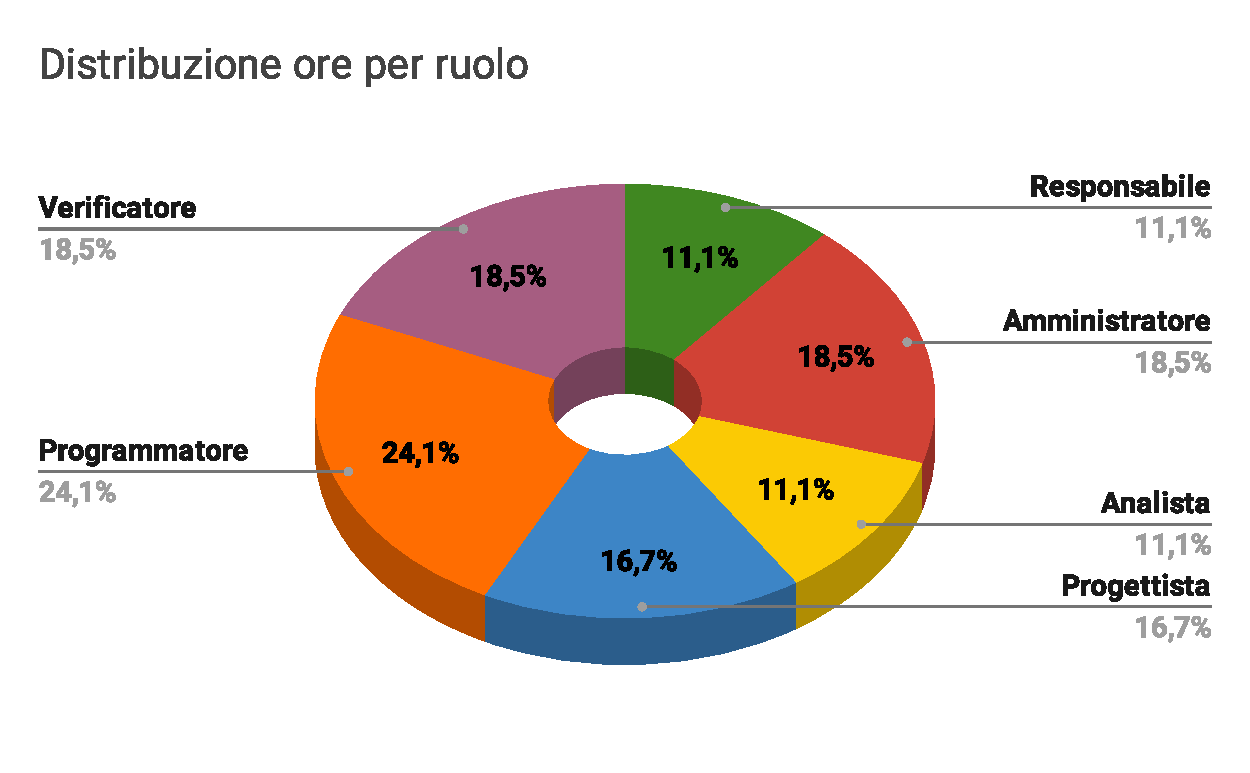
\includegraphics[width=0.90\textwidth]{assets/Preventivo/Sprint-4/distribuzione_ore_ruolo.pdf}
  \caption{Sprint 4 - Areogramma della distribuzione oraria per ruolo}
\end{figure}

\begin{minipage}{\textwidth}
Di seguito è riportato il preventivo economico del quarto \glossario{sprint}:
\begin{table}[H]
  \centering
  \begin{tabular}{|c|c|c|}
    \hline
    \multicolumn{3}{|c|}{\textbf{Preventivo economico}} \\
    \hline
    \textbf{Ruolo} & \textbf{Ore per ruolo} & \textbf{Costo (in \texteuro)} \\
    \hline
    Responsabile & 6 & 180,00 \\
    \hline
    Amministratore & 10 & 200,00 \\
    \hline
    Analista & 6 & 150,00 \\
    \hline
    Progettista & 9 & 225,00 \\
    \hline
    Programmatore & 13 & 195,00 \\
    \hline
    Verificatore & 10 & 150,00 \\
    \hline
    \textbf{Totale} & 54 & \textbf{1.100,00} \\
    \hline
  \end{tabular}
  \caption{Sprint 4 - Preventivo economico}
\end{table}
\end{minipage}
\subsubsection{Sprint 5: da 2024-06-05 a 2024-06-14}
Durante lo \glossario{sprint} precedente, il team ha approfondito ulteriormente i framework \glossario{Flask} e \glossario{Vue.js}, che nel corso di questo sprint saranno utilizzati in sinergia per integrare \glossario{front-end} e \glossario{back-end}.
Inoltre sarà programmato un incontro con il Professore Riccardo Cardin per chiarimenti sulle tecnologie scelte. Gli obiettivi sono stati definiti in vista dell'avvicinamento dell'RTB. 


\paragraph{Obiettivi}
\begin{itemize}
  \item Aggiornamento del \PdP con particolare attenzione sul preventivo a finire dello sprint 4 e la redistribuzione delle ore per ruolo;
  \item Proseguire con la stesura delle \NdP;
  \item Programmare un incontro con il Professore Riccardo Cardin per dubbi sulle tecnologie;
  \item Stesura dei verbali interni ed esterni;
  \item Ampliamento dei casi d'uso nell' \AdR con estensioni ed errori ed inserimento dei grafici dei \glossario{casi d'uso} rimanenti;
  \item Configurazione \glossario{Flask} - \glossario{Vue.js};
  \item Integrazione \glossario{back-end} e \glossario{front-end};
  \item Connessione al database con \glossario{Flask};
  \item Gestione \glossario{CRUD} dizionario dati in backend;
  \item Ultimi approfondimenti del funzionamento di txtai;
  \item Progettazione generale struttura front-end;
  \item Visualizzazione \glossario{log} e struttura del \glossario{dizionario dati} lato \glossario{front-end}.
\end{itemize}

\vspace{0.5\baselineskip}
\par [Inserire Gantt]
\subsection{Sesto sprint}

\begin{minipage}{\textwidth}
  Di seguito è riportata la distribuzione delle ore per ciascun membro del team, accumulate in totali per persona e per ruolo:
  \begin{table}[H]
    \begin{tabularx}{\textwidth}{|c|*{6}{>{\centering}X|}c|}
      \hline
      \multicolumn{8}{|c|}{\textbf{Consuntivo orario}} \\
      \hline
      \textbf{Membro del team} & \textbf{Re} & \textbf{Am} & \textbf{An} & \textbf{Pt} & \textbf{Pr} & \textbf{Ve} & \textbf{Totale per persona} \\
      \hline
      Cavalli Riccardo & 0 & 1 & 3 & 0 & 0 & 0 & 4 \\
      \hline
      Pianon Raul & 0 & 3 & 1 & 0 & 0 & 0 & 4 \\
      \hline
      Dall’Amico Martina & 1 & 0 & 0 & 0 & 3 & 1 & 5 \\
      \hline
      Cristo Marco & 0 & 1 & 1 & 0 & 0 & 1 & 3 \\
      \hline
      Lewental Sebastiano & 3 & 0 & 0 & 0 & 1 & 0 & 4 \\
      \hline
      Zecchinato Mattia & 0 & 2 & 0 & 0 & 2 & 1 & 5 \\
      \hline
      Stocco Tommaso & 0 & 0 & 0 & 0 & 2 & 1 & 3 \\
      \hline
      \textbf{Totale ore per ruolo} & 4 & 7 & 5 & 0 & 8 & 4 & \textbf{28} \\
      \hline
    \end{tabularx}
    \caption{Sprint 6 - Consuntivo orario}
  \end{table}
  \end{minipage}

  \begin{figure}[H]
    \centering
    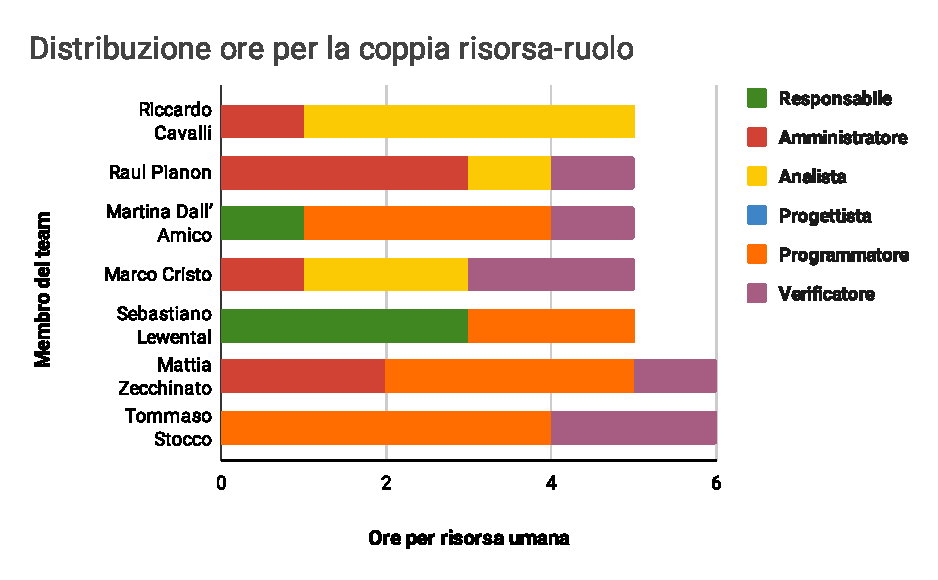
\includegraphics[width=0.90\textwidth]{assets/Consuntivo/Sprint-6/distribuzione_ore_risorsa_ruolo.pdf}
    \caption{Sprint 6 - Istogramma della distribuzione oraria per la coppia risorsa-ruolo}
  \end{figure}

  \begin{figure}[H]
    \centering
    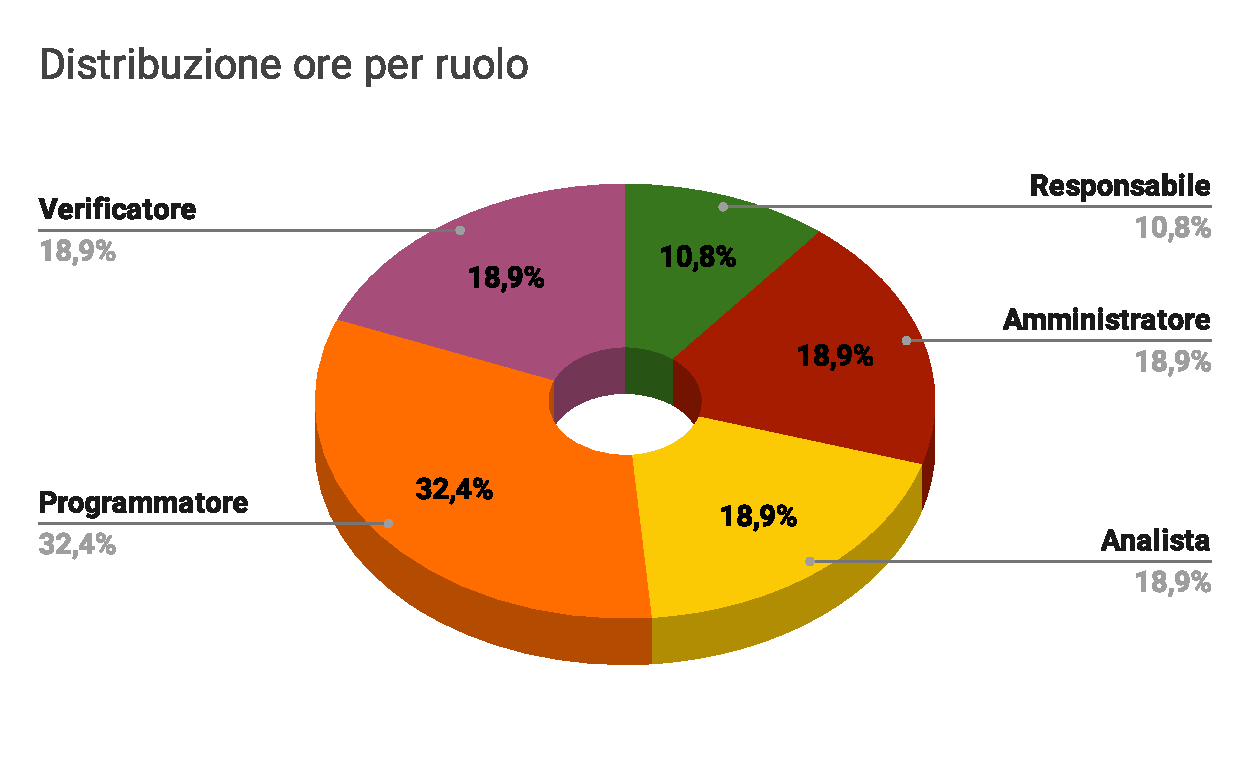
\includegraphics[width=0.90\textwidth]{assets/Consuntivo/Sprint-6/distribuzione_ore_ruolo.pdf}
    \caption{Sprint 6 - Areogramma della distribuzione oraria per ruolo}
  \end{figure}

  \begin{minipage}{\textwidth}
  Di seguito è riportato il consuntivo economico del sesto \glossario{sprint}:
  \begin{table}[H]
  \begin{adjustwidth}{-0.5cm}{-0.5cm}
    \centering
    \begin{tabular}{|P{2.9cm}|P{2.3cm}|P{2.5cm}|P{2.3cm}|>{\arraybackslash}P{2.5cm}|}
      \hline
      \multicolumn{5}{|c|}{\textbf{Consuntivo economico}} \\
      \hline
      \textbf{Ruolo} & \textbf{Ore per ruolo} & \textbf{Delta ore preventivo - consuntivo} & \textbf{Costo (in \texteuro)} & \textbf{Delta costo preventivo - consuntivo (in \texteuro)} \\
      \hline
      Responsabile & 4 & -1 & 120,00 & -30,00 \\ \hline
      Amministratore & 7 & 1 & 140,00 & 20,00 \\ \hline
      Analista & 5 & 1 & 125,00 & 25,00 \\ \hline
      Progettista & 0 & 0 & 0,00 & 0,00 \\ \hline
      Programmatore & 8 & 1 & 120,00 & 15,00 \\ \hline
      Verificatore & 4 & 0 & 60,00 & 0,00 \\ \hline
      \textbf{Totale} & \textbf{28} & 2 & \textbf{565,00} & 30,00 \\ \hline
      \textbf{Restante} & 380 & / & 7.515,00 & / \\ \hline
      \textbf{Sprint pregressi} & 236 & / & 4.905,00 & / \\ \hline
    \end{tabular}
    \caption{Sprint 6 - Consuntivo economico}
  \end{adjustwidth}
  \end{table}
  \end{minipage}

  \begin{figure}[H]
    \centering
    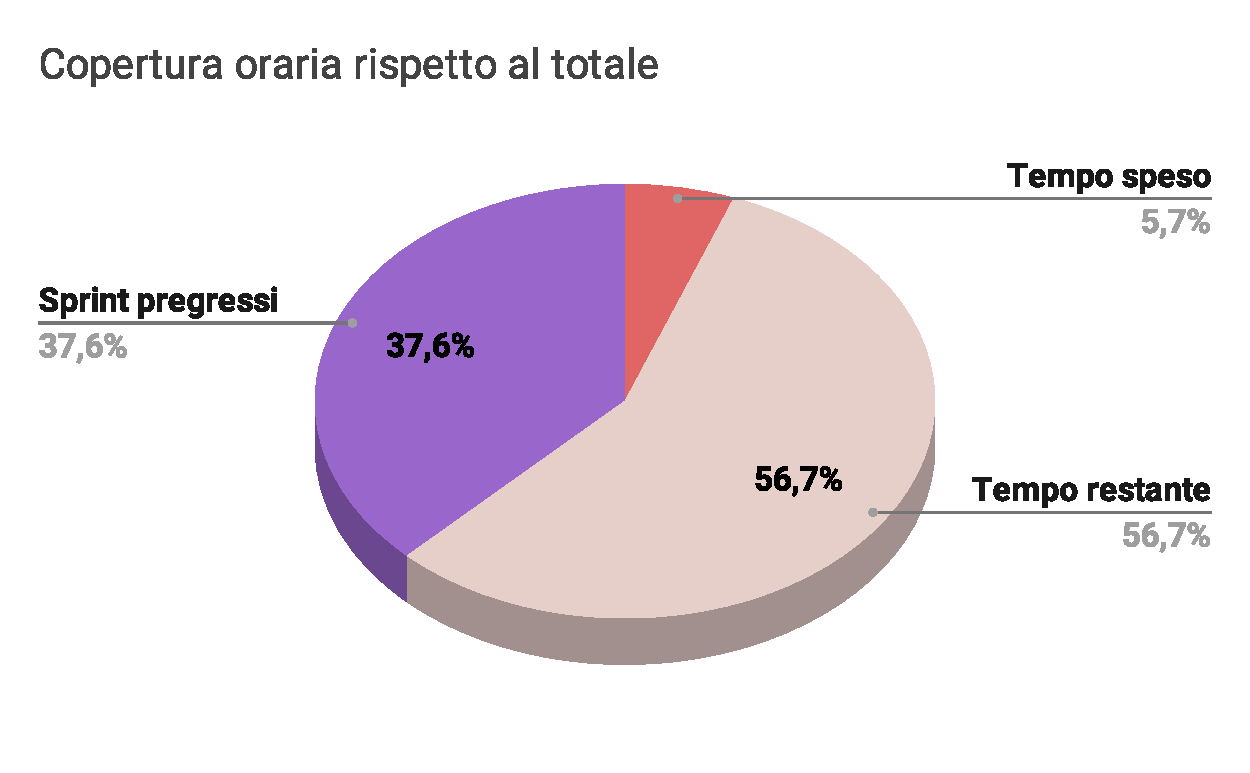
\includegraphics[width=0.90\textwidth]{assets/Consuntivo/Sprint-6/copertura_oraria.pdf}
    \caption{Sprint 6 - Areogramma del tempo speso (in ore) rispetto al totale}
  \end{figure}

  \begin{figure}[H]
    \centering
    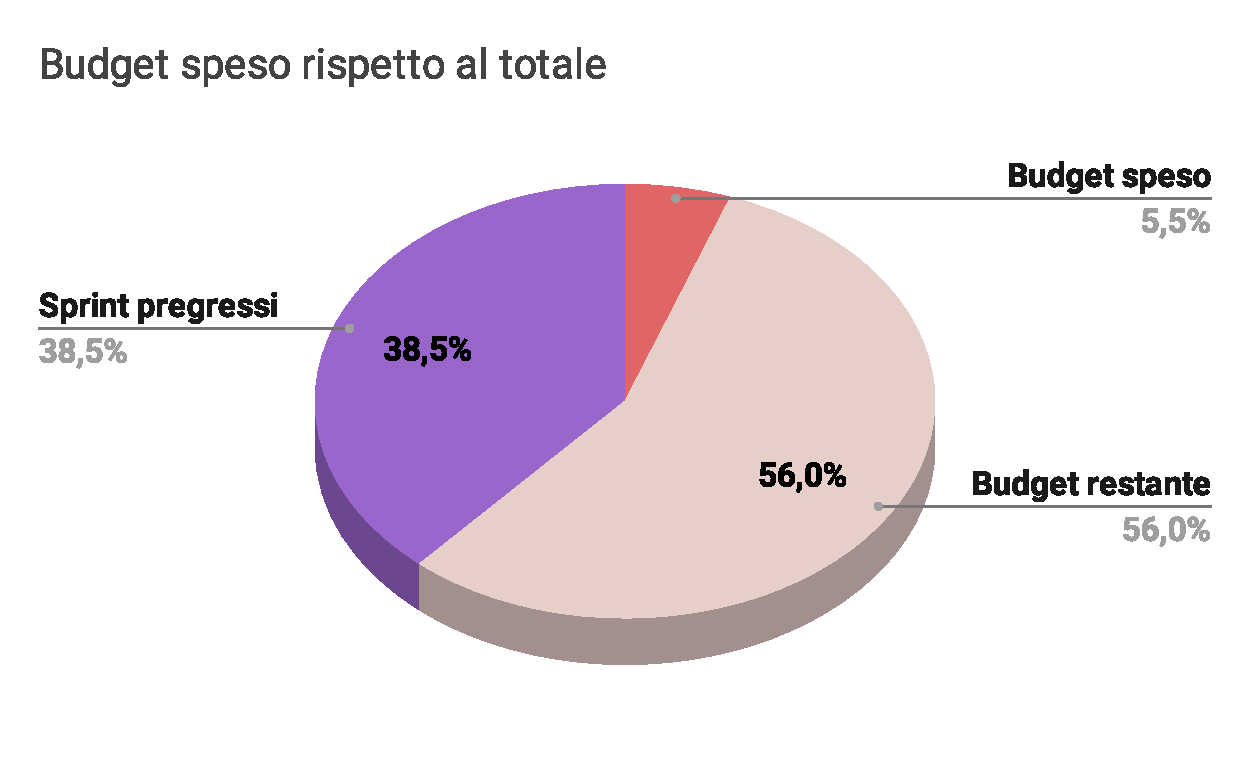
\includegraphics[width=0.90\textwidth]{assets/Consuntivo/Sprint-6/budget_speso.pdf}
    \caption{Sprint 6 - Areogramma del budget speso rispetto al totale}
  \end{figure}

  \begin{minipage}{\textwidth}
    Di seguito sono riportate le ore rimanenti per la coppia risorsa-ruolo:
    \begin{table}[H]
      \begin{tabularx}{\textwidth}{|c|*{6}{>{\centering}X|}c|}
        \hline
        \multicolumn{8}{|c|}{\textbf{Ore rimanenti per la coppia risorsa-ruolo}} \\
        \hline
        \textbf{Membro del team} & \textbf{Re} & \textbf{Am} & \textbf{An} & \textbf{Pt} & \textbf{Pr} & \textbf{Ve} & \textbf{Totale per persona} \\
        \hline
        Cavalli Riccardo & 0 & 0 & 4 & 14 & 16 & 15 & 49 \\
        \hline
        Pianon Raul & 2 & 7 & 1 & 20 & 10 & 12 & 52 \\
        \hline
        Dall’Amico Martina & 5 & 2 & 1 & 14 & 19 & 12 & 53 \\
        \hline
        Cristo Marco & 2 & 9 & 1 & 17 & 10 & 14 & 53 \\
        \hline
        Lewental Sebastiano & 6 & 4 & 2 & 11 & 17 & 15 & 55 \\
        \hline
        Zecchinato Mattia & 9 & 6 & 3 & 11 & 14 & 14 & 57 \\
        \hline
        Stocco Tommaso & 5 & 4 & 3 & 20 & 11 & 18 & 61 \\
        \hline
        \textbf{Totale ore per ruolo} & 29 & 32 & 15 & 107 & 97 & 100 & \textbf{380} \\
        \hline
      \end{tabularx}
      \caption{Sprint 6 - Ore rimanenti per la coppia risorsa-ruolo}
    \end{table}
  \end{minipage}

\subsubsection{Revisione delle attività}

Nell'arco del sesto \glossario{sprint}, il team ha svolto le seguenti attività:
\begin{itemize}
    \item Stesura dei verbali interni ed esterni;
    \item Miglioramento della struttura dei \glossario{casi d'uso} nell’\AdR;
    \item Revisione dei grafici nell’\AdR;
    \item Ampliamento dei casi d’uso con la gestione del \glossario{debug} e degli errori;
    \item Aggiornamento del \PdP; (stesura delle sezioni incomplete e revi-sione dei consuntivi precedenti);
    \item Stesura della dashboard di valutazione della qualità nel Piano di Qualifica;
    \item Inserimento dei grafici nel Piano di Qualifica;
    \item Creazione componente di login funzionante;
    \item Sviluppo delle pagine \glossario{front-end} (chat, gestione dei \glossario{dizionari dati} e debug).
\end{itemize}

\subsubsection{Retrospettiva}

\par Di seguito sono riportati i risultati del questionario di valutazione dello \glossario{sprint}:
\begin{itemize}
  \item Organizzazione dello \glossario{sprint}\ - Valutazione: 8;
  \item Conduzione dei meeting interni - Valutazione: 8;
  \item Conduzione dei meeting esterni - Valutazione: 8;
  \item Impegno e partecipazione dei singoli membri - Valutazione: 7;
  \item La quasi totalità dei membri del team era a conoscenza delle proprie mansioni;
  \item La numerosità delle riunioni è risultata adeguata per tutti i membri del gruppo;
  \item Le riunioni sono state organizzate quasi sempre con il giusto preavviso;
  \item Il rapporto ore spese/ore produttive si sta notevolmente equilibrando;
  \item La produttività è stata ragioneole considerando le criticità dell'imminente sessione;
  \item È diffusa l'idea di programmare incontri in presenza più frequenti.
\end{itemize}

\vspace{0.5\baselineskip}
\par A seguire le \textbf{analisi a posteriori} del sesto \glossario{sprint}:
\begin{itemize}
  \item In seguito ad un incontro in presenza avvenuto durante questo \glossario{sprint}, il team ha notato quanto più efficace risulti questa modalità di lavoro rispetto a quella a distanza, evidenziata dalla quantità di \glossario{pull request} avvenute e risolte in tale occasione;
  \item Le precedenti tecnologie individuate per la parte di \glossario{backend} sono risultate troppo complesse per lo sviluppo in essere, quindi è stata decisa un'ulteriore modifica della libreria, col passaggio a \glossario{FastAPI};
  \item La sessione di esami ha impattato sulla quantità di lavoro svolto, come previsto.
\end{itemize}

\subsubsection{Aggiornamento pianificazione e preventivo}
\par Il team ha definito un piano d'azione per migliorare l'organizzazione e la produttività del prossimo \glossario{sprint}:
\begin{itemize}
  \item Pianificare incontri in presenza con frequenza maggiore, di almeno un incontro ogni due settimane;
\end{itemize}

\paragraph*{Pianificazione futura:}
\par Come riportato nell'analisi a posteriori, il team ha deciso di aumentare il numero di riunioni in presenza.
Inoltre si è deciso di mantenere moderata la quantità di ore assegnate a ciascun membro del team, in modo da continuare a garantire un equilibrio tra lavoro e studio.

\paragraph*{Preventivo "a finire" (\sezione{sec:stima_temporale}):}
\par L'avanzamento dello stato prodotto porta a stabilire la prossimità della revisione RTB, che avverrà tuttavia dopo la sessione di esami.

\paragraph*{Gestione dei rischi (\sezione{sec:analisi_rischi}):}
\par Nel corso del sesto \glossario{sprint}, il seguente rischio si è presentato ed è stato gestito correttamente:
\begin{itemize}
  \item \textbf{Rischi relativi a rallentamenti}: In prossimità della sessione di esami, il team ha avuto difficoltà a conciliare l'avanzamento del progetto e lo studio personale; pertanto, le ore produttive individuali sono state ridotte. Trattandosi di un rischio preventivato, la data di consegna non ha subito alterazioni in quanto era stata pianificata in modo adeguato.
\end{itemize}

\subsubsection{Sprint 7: da 2024-06-25 a 2024-07-02}
Il team in vista della RTB si appresta a concludere le attività di programmazione relative al \glossario{PoC} e nell'ultimare le sezioni incomplete dei documenti, focalizzandosi maggiormente sulla sezione documentale  prima della consegna.


\paragraph{Obiettivi}
\begin{itemize}
  \item Revisione consuntivi \PdP;
  \item Aggiunta metriche alle \NdP;
  \item Completamento sezioni incomplete \NdP;
  \item Stesura sezione test nel \PdQ;
  \item Stesura dei verbali interni;
  \item Gestione stato Utente/Tecnico a \glossario{front-end};
  \item Creazione interfaccia Chat a \glossario{front-end};
  \item Implementazione funzioni per generare il \glossario{prompt} e mostrarlo a \glossario{front-end}.
\end{itemize}

\vspace{0.5\baselineskip}
\par [Inserire Gantt]

\subsection{Ottavo sprint}

\begin{minipage}{\textwidth}
  Di seguito è riportata la distribuzione delle ore per ciascun membro del team, accumulate in totali per persona e per ruolo:
  \begin{table}[H]
    \begin{tabularx}{\textwidth}{|c|*{6}{>{\centering}X|}c|}
      \hline
      \multicolumn{8}{|c|}{\textbf{Consuntivo orario}} \\
      \hline
      \textbf{Membro del team} & \textbf{Re} & \textbf{Am} & \textbf{An} & \textbf{Pt} & \textbf{Pr} & \textbf{Ve} & \textbf{Totale per persona} \\
      \hline
      Riccardo Cavalli & 0 & 0 & 0 & 0 & 2 & 2 & 4 \\
      \hline
      Raul Pianon & 0 & 2 & 0 & 0 & 0 & 2 & 4 \\
      \hline
      Martina Dall'Amico & 2 & 1 & 0 & 0 & 0 & 1 & 4 \\
      \hline
      Marco Cristo & 0 & 2 & 0 & 0 & 0 & 2 & 4 \\
      \hline
      Sebastiano Lewental & 0 & 0 & 1 & 0 & 1 & 2 & 4 \\
      \hline
      Mattia Zecchinato & 2 & 1 & 0 & 0 & 1 & 0 & 4 \\
      \hline
      Tommaso Stocco & 0 & 0 & 0 & 0 & 0 & 0 & 3 \\
      \hline
      \textbf{Totale ore per ruolo} & 4 & 6 & 1 & 0 & 4 & 12 & \textbf{27} \\
      \hline
    \end{tabularx}
    \caption{Sprint 8 - Consuntivo orario}
  \end{table}
  \end{minipage}

  \begin{figure}[H]
    \centering
    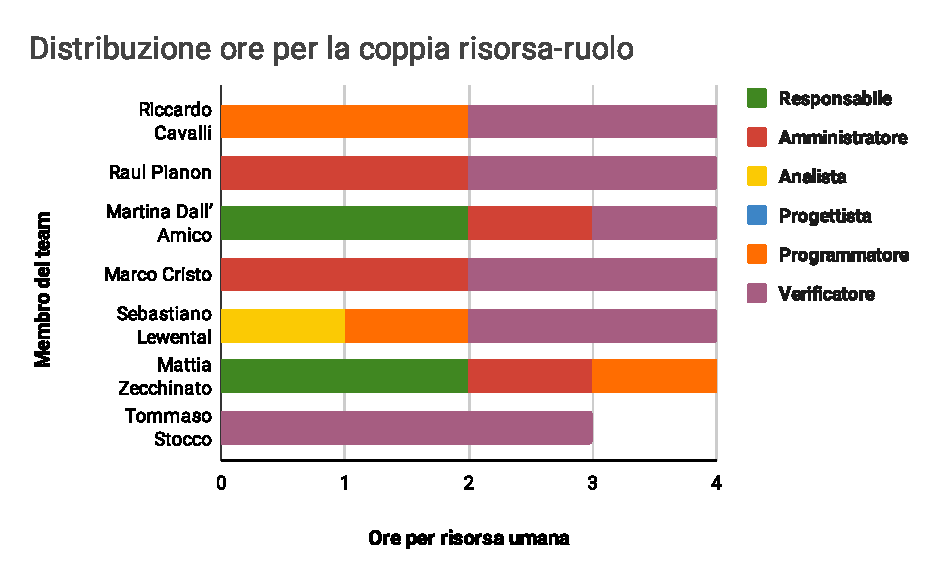
\includegraphics[width=0.90\textwidth]{assets/Consuntivo/Sprint-8/distribuzione_ore_risorsa_ruolo.pdf}
    \caption{Sprint 8 - Istogramma della distribuzione oraria per la coppia risorsa-ruolo}
  \end{figure}

  \begin{figure}[H]
    \centering
    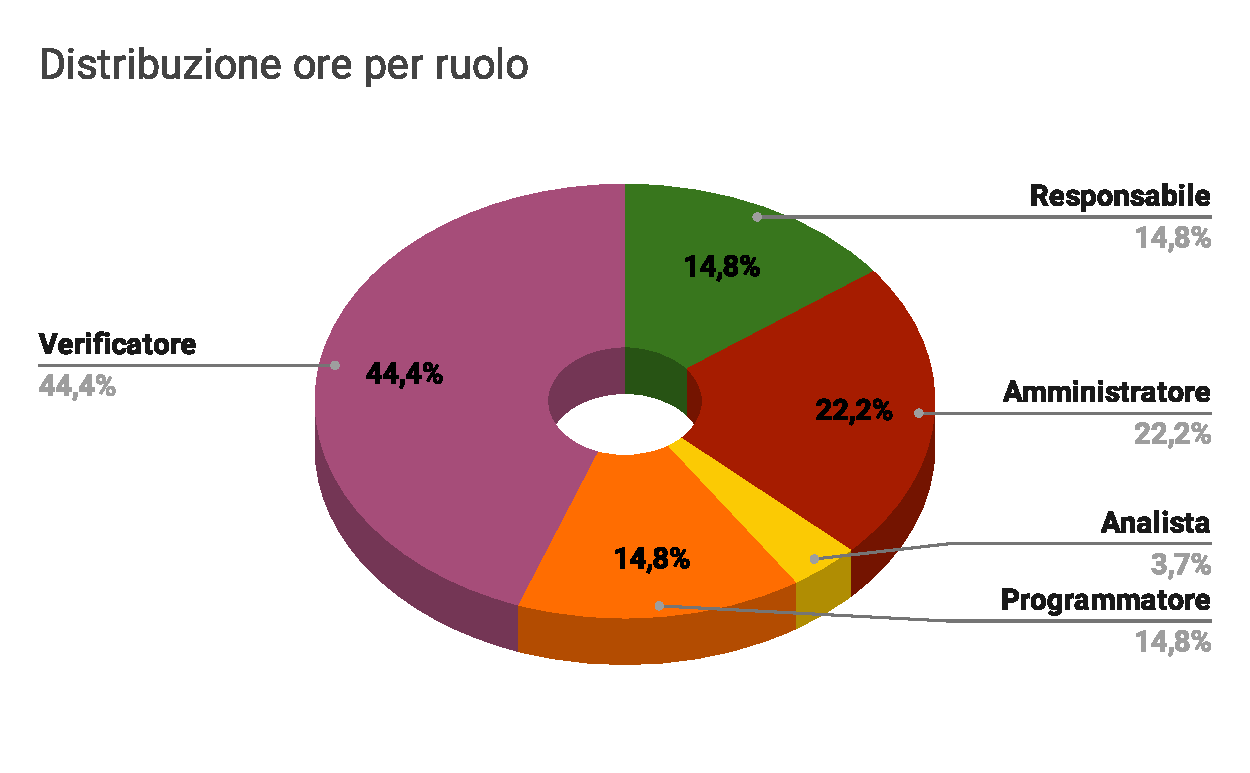
\includegraphics[width=0.90\textwidth]{assets/Consuntivo/Sprint-8/distribuzione_ore_ruolo.pdf}
    \caption{Sprint 8 - Areogramma della distribuzione oraria per ruolo}
  \end{figure}

  \begin{minipage}{\textwidth}
  Di seguito è riportato il consuntivo economico dell'ottavo \glossario{sprint}:
  \begin{table}[H]
  \begin{adjustwidth}{-0.5cm}{-0.5cm}
    \centering
    \begin{tabular}{|P{2.9cm}|P{2.3cm}|P{2.5cm}|P{2.3cm}|>{\arraybackslash}P{2.5cm}|}
      \hline
      \multicolumn{5}{|c|}{\textbf{Consuntivo economico}} \\
      \hline
      \textbf{Ruolo} & \textbf{Ore per ruolo} & \textbf{Delta ore preventivo - consuntivo} & \textbf{Costo (in \texteuro)} & \textbf{Delta costo preventivo - consuntivo (in \texteuro)} \\
      \hline
      \Responsabile[U]{} & 4 & -1 & 120,00 & -30,00 \\ \hline
      \Amministratore[U]{} & 6 & 1 & 120,00 & 20,00 \\ \hline
      \Analista[U]{} & 1 & 1 & 25,00 & 25,00 \\ \hline
      \Progettista[U]{} & 0 & 0 & 0,00 & 0,00 \\ \hline
      \Programmatore[U]{} & 4 & 0 & 60,00 & 0,00 \\ \hline
      \Verificatore[U]{} & 12 & 0 & 180,00 & 0,00 \\ \hline
      \textbf{Totale} & \textbf{27} & 1 & \textbf{505,00} & 15,00 \\ \hline
      \textbf{Restante} & 311 & / & 6.270,00 & / \\ \hline
      \textbf{Sprint pregressi} & 308 & / & 6.245,00 & / \\ \hline
    \end{tabular}
    \caption{Sprint 8 - Consuntivo economico}
  \end{adjustwidth}
  \end{table}
  \end{minipage}

  \begin{figure}[H]
    \centering
    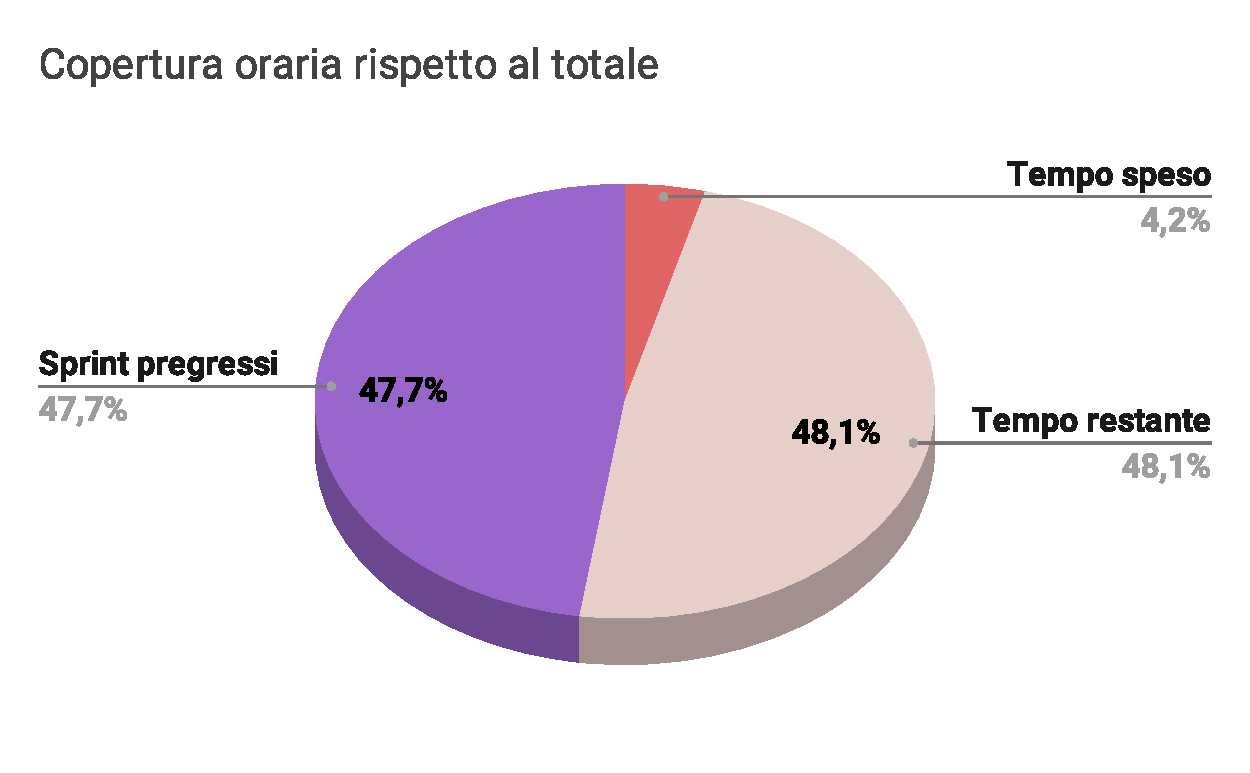
\includegraphics[width=0.90\textwidth]{assets/Consuntivo/Sprint-8/copertura_oraria.pdf}
    \caption{Sprint 8 - Areogramma del tempo speso (in ore) rispetto al totale}
  \end{figure}

  \begin{figure}[H]
    \centering
    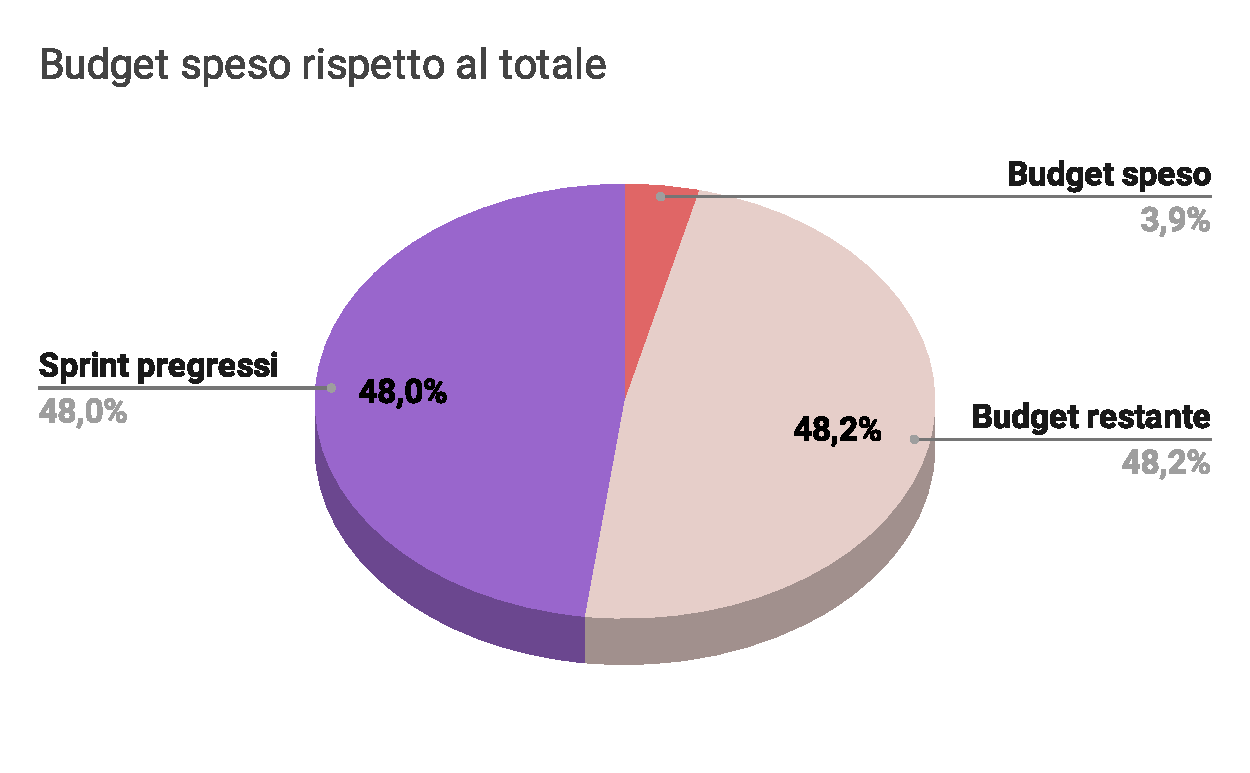
\includegraphics[width=0.90\textwidth]{assets/Consuntivo/Sprint-8/budget_speso.pdf}
    \caption{Sprint 8 - Areogramma del budget speso rispetto al totale}
  \end{figure}

  \begin{minipage}{\textwidth}
    Di seguito sono riportate le ore rimanenti per la coppia risorsa-ruolo:
    \begin{table}[H]
      \begin{tabularx}{\textwidth}{|c|*{6}{>{\centering}X|}c|}
        \hline
        \multicolumn{8}{|c|}{\textbf{Ore rimanenti per la coppia risorsa-ruolo}} \\
        \hline
        \textbf{Membro del team} & \textbf{Re} & \textbf{Am} & \textbf{An} & \textbf{Pt} & \textbf{Pr} & \textbf{Ve} & \textbf{Totale per persona} \\
        \hline
        Riccardo Cavalli & 0 & 1 & 3 & 14 & 11 & 11 & 40 \\
        \hline
        Raul Pianon & 2 & 3 & 1 & 20 & 10 & 7 & 43 \\
        \hline
        Martina Dall'Amico & 3 & 1 & 1 & 14 & 16 & 11 & 46 \\
        \hline
        Marco Cristo & 2 & 6 & 0 & 17 & 10 & 9 & 44 \\
        \hline
        Sebastiano Lewental & 5 & 4 & 1 & 11 & 11 & 13 & 45 \\
        \hline
        Mattia Zecchinato & 5 & 2 & 3 & 11 & 11 & 13 & 45 \\
        \hline
        Tommaso Stocco & 5 & 0 & 3 & 20 & 9 & 11 & 48 \\
        \hline
        \textbf{Totale ore per ruolo} & 22 & 17 & 12 & 107 & 78 & 75 & \textbf{311} \\
        \hline
      \end{tabularx}
      \caption{Sprint 8 - Ore rimanenti per la coppia risorsa-ruolo}
    \end{table}
  \end{minipage}

\subsubsection{Revisione delle attività}

Nell'arco dell'ottavo \glossario{sprint}, il team ha svolto le seguenti attività:
\begin{itemize}
  \item Aggiornamento della documentazione in preparazione alla prima fase della revisione \glossario{RTB};
  \item Completamento \glossario{PoC};
  \item Revisione delle metriche di processo e di prodotto;
  \item Suddivisione delle metriche in base all'obiettivo.
\end{itemize}

\subsubsection{Retrospettiva}

\par Di seguito sono riportati i risultati del questionario di valutazione dello \glossario{sprint}:
\begin{itemize}
  \item Organizzazione dello sprint - Valutazione: 8;
  \item Conduzione dei meeting interni - Valutazione: 8;
  \item Conduzione dei meeting esterni - Valutazione: 8;
  \item Impegno e partecipazione dei singoli membri - Valutazione: 3;
  \item La quasi totalità dei membri del team era a conoscenza delle proprie mansioni;
  \item La numerosità delle riunioni è risultata adeguata per tutti i membri del gruppo;
  \item Le riunioni sono state organizzate quasi sempre con il giusto preavviso;
  \item Il rapporto ore spese/ore produttive si sta notevolmente equilibrando;
  \item La produttività è stata ragioneole considerando le criticità della sessione.
\end{itemize}

\vspace{0.5\baselineskip}
\par A seguire le \textbf{analisi a posteriori} dell'ottavo \glossario{sprint}:
\begin{itemize}
  \item La sessione di esami ha impattato sulla quantità di lavoro svolto, come previsto.
  \item Così come nello \glossario{sprint} precedente, a causa sessione, è stato difficile organizzare incontri frequenti con la partecipazione completa del gruppo. Le riunioni in presenza, naturalmente più sporadiche e ricche in intensità e durata, si sono rivelate particolarmente proficue; in questo modo il team ha potuto collaborare con più efficienza sullo sviluppo tecnologico dell'applicativo, oltre che sulla preparazione della presentazione dei contenuti per la \RTB.
  \item L'esperienza relativa agli ultimi \glossario{sprint} della durata di circa una settimana ha concesso ai membri del team una maggiore consapevolezza nella propria autogestione nel corso della sessione. Resta tuttavia la decisione di ripianificare gli \glossario{sprint} seguenti il termine della sessione a una durata di due settimane per facilitare una migliore organizzazione complessiva.
\end{itemize}

\subsubsection{Aggiornamento pianificazione e preventivo}
\paragraph*{Pianificazione futura:}
\par Si è deciso di mantenere moderata la quantità di ore assegnate a ciascun membro del team, in modo da continuare a garantire un equilibrio tra lavoro e studio. Confermando lo stato del progetto, si è deciso di fissare gli appuntamenti relativi alla \glossario{RTB} nel prossimo sprint.

\paragraph*{Preventivo "a finire" (\sezione{sec:stima_temporale}):}
\par L'avanzamento dello stato del progetto porta a stabilire l'organizzazione della revisione RTB durante il prossimo \glossario{sprint}.

\paragraph*{Gestione dei rischi (\sezione{sec:analisi_rischi}):}
\vspace{0.5\baselineskip}
\par Durante l'ottavo \glossario{sprint}, i seguenti rischi sono stati gestiti con successo:
\begin{itemize}
  \item \textbf{RO1 - Periodi di rallentamento}: il \Responsabile{} ha riallocato le risorse e riassegnato le attività in tutti i giorni precedenti un esame;
  \item \textbf{RP1 - Questioni personali}: alcuni membri del gruppo hanno dovuto affrontare questioni personali che hanno impattato sulla loro partecipazione alle attività. Tuttavia, la flessibilità del team ha permesso di riallocare le risorse in modo da garantire il rispetto delle scadenze;
  \item \textbf{RT3 - Malfunzionamenti software}: gli errori sono stati risolti mediante la ricostruzione delle immagini Docker, in conformità con le specifiche definite nel README caricato nel repository ChatSQL.
\end{itemize}

\subsubsection{Sprint 9: da 2024-07-11 a 2024-07-20}
\begin{minipage}{\textwidth}
Di seguito è riportata la distribuzione delle ore per ciascun membro del team, accumulate in totali per persona e per ruolo:
\begin{table}[H]
  \begin{tabularx}{\textwidth}{|c|*{6}{>{\centering}X|}c|}
    \hline
    \multicolumn{8}{|c|}{\textbf{Preventivo orario}} \\
    \hline
    \textbf{Membro del team} & \textbf{Re} & \textbf{Am} & \textbf{An} & \textbf{Pt} & \textbf{Pr} & \textbf{Ve} & \textbf{Totale per persona} \\
    \hline
    Riccardo Cavalli & 0 & 0 & 0 & 1 & 1 & 2 & 4 \\
    \hline
    Raul Pianon & 0 & 2 & 0 & 1 & 0 & 1 & 4 \\
    \hline
    Martina Dall'Amico & 1 & 0 & 0 & 0 & 0 & 3 & 4 \\
    \hline
    Marco Cristo & 0 & 2 & 0 & 0 & 0 & 2 & 4 \\
    \hline
    Sebastiano Lewental & 2 & 0 & 0 & 0 & 0 & 2 & 4 \\
    \hline
    Mattia Zecchinato & 0 & 0 & 0 & 2 & 0 & 2 & 4 \\
    \hline
    Tommaso Stocco & 0 & 0 & 0 & 1 & 0 & 3 & 4 \\
    \hline
    \textbf{Totale ore per ruolo} & 3 & 4 & 0 & 5 & 1 & 15 & \textbf{28} \\
    \hline
  \end{tabularx}
  \caption{Sprint 9 - Preventivo orario}
\end{table}
\end{minipage}

\begin{figure}[H]
  \centering
  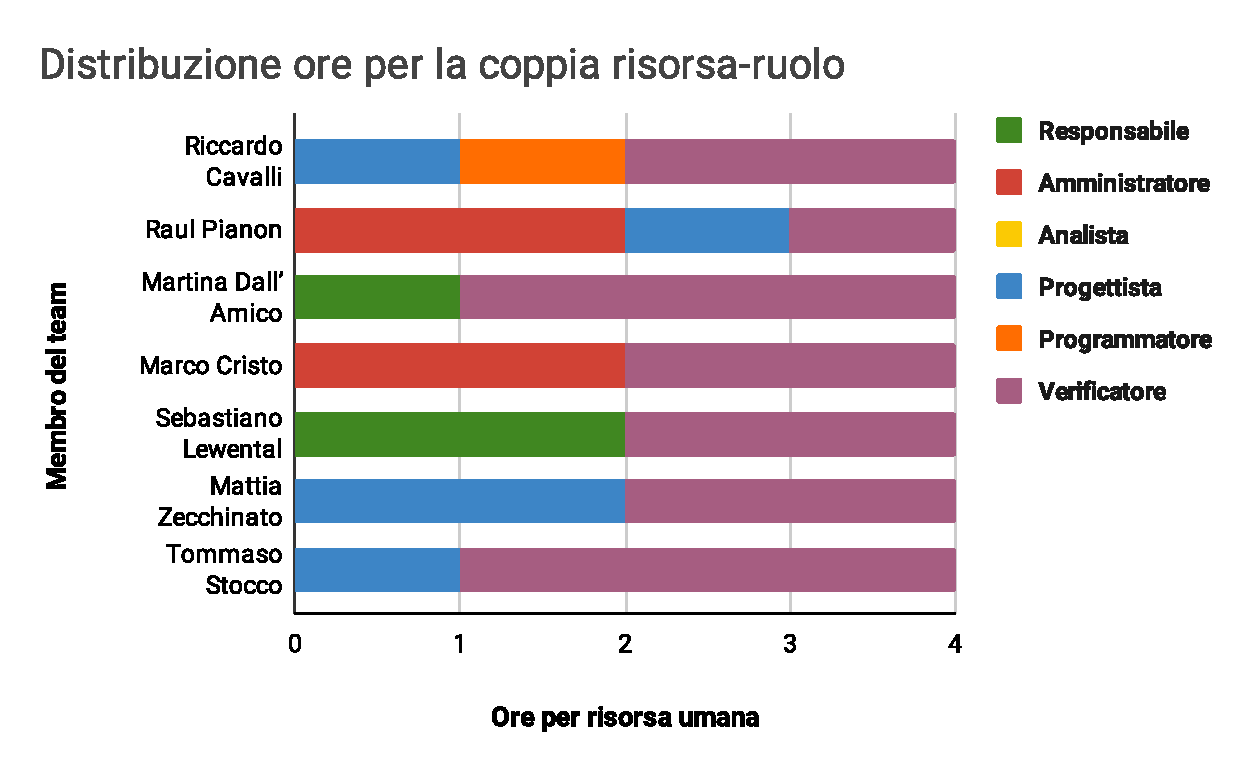
\includegraphics[width=0.90\textwidth]{assets/Preventivo/Sprint-9/distribuzione_ore_risorsa_ruolo.pdf}
  \caption{Sprint 9 - Istogramma della distribuzione oraria per la coppia risorsa-ruolo}
\end{figure}

\begin{figure}[H]
  \centering
  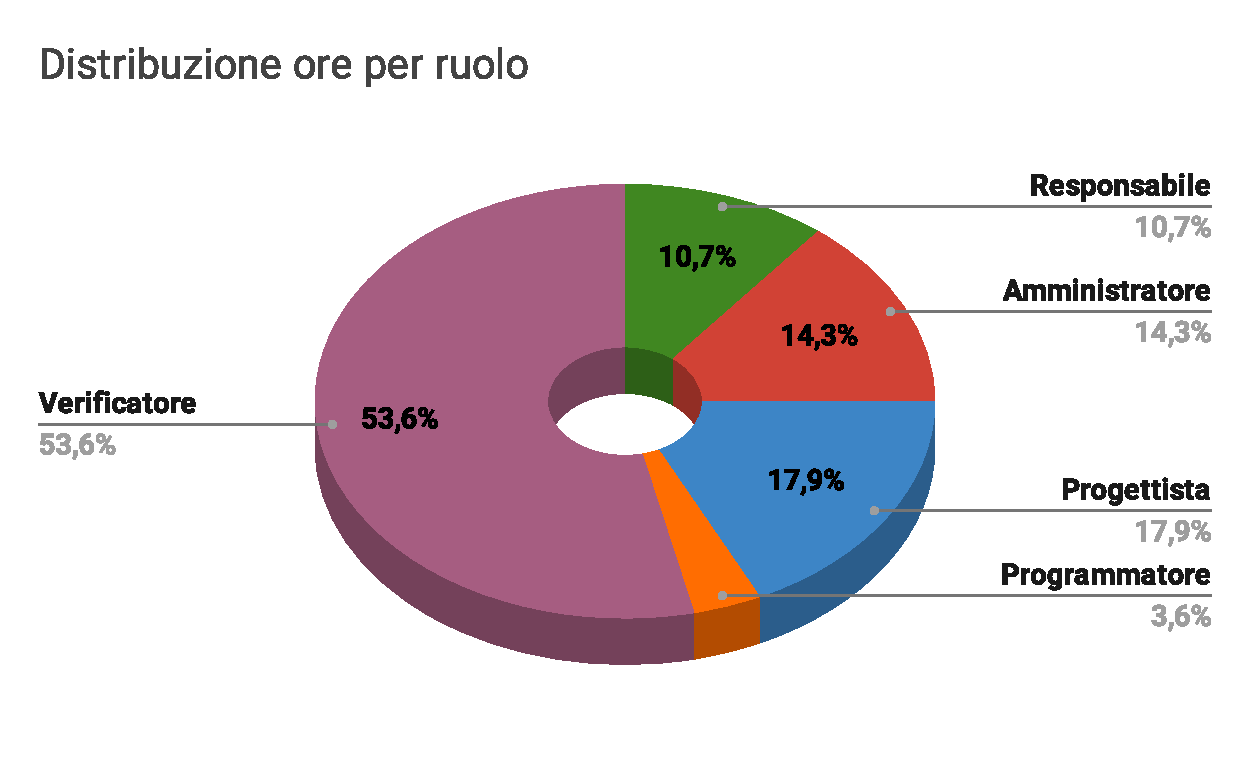
\includegraphics[width=0.90\textwidth]{assets/Preventivo/Sprint-9/distribuzione_ore_ruolo.pdf}
  \caption{Sprint 9 - Areogramma della distribuzione oraria per ruolo}
\end{figure}

\begin{minipage}{\textwidth}
Di seguito è riportato il preventivo economico dell'ottavo \glossario{sprint}:
\begin{table}[H]
  \centering
  \begin{tabular}{|c|c|c|}
    \hline
    \multicolumn{3}{|c|}{\textbf{Preventivo economico}} \\
    \hline
    \textbf{Ruolo} & \textbf{Ore per ruolo} & \textbf{Costo (in \texteuro)} \\
    \hline
    Responsabile & 3 & 90,00 \\
    \hline
    Amministratore & 4 & 80,00 \\
    \hline
    Analista & 0 & 0,00 \\
    \hline
    Progettista & 5 & 125,00 \\
    \hline
    Programmatore & 1 & 15,00 \\
    \hline
    Verificatore & 15 & 225,00 \\
    \hline
    \textbf{Totale} & 28 & \textbf{535,00} \\
    \hline
  \end{tabular}
  \caption{Sprint 9 - Preventivo economico}
\end{table}
\end{minipage}

\subsection{Decimo sprint}

\begin{minipage}{\textwidth}
  Di seguito è riportata la distribuzione delle ore per ciascun membro del team, accumulate in totali per persona e per ruolo:
  \begin{table}[H]
    \begin{tabularx}{\textwidth}{|c|*{6}{>{\centering}X|}c|}
      \hline
      \multicolumn{8}{|c|}{\textbf{Consuntivo orario}} \\
      \hline
      \textbf{Membro del team} & \textbf{Re} & \textbf{Am} & \textbf{An} & \textbf{Pt} & \textbf{Pr} & \textbf{Ve} & \textbf{Totale per persona} \\
      \hline
      Riccardo Cavalli & 0 & 0 & 0 & 5 & 1 & 3 & 9 \\
      \hline
      Raul Pianon & 0 & 0 & 0 & 6 & 1 & 2 & 9 \\
      \hline
      Martina Dall'Amico & 0 & 0 & 0 & 2 & 6 & 1 & 9 \\
      \hline
      Marco Cristo & 1 & 0 & 0 & 6 & 0 & 2 & 9 \\
      \hline
      Sebastiano Lewental & 1 & 1 & 0 & 4 & 0 & 3 & 9 \\
      \hline
      Mattia Zecchinato & 0 & 0 & 1 & 0 & 5 & 3 & 9 \\
      \hline
      Tommaso Stocco & 2 & 0 & 0 & 4 & 0 & 3 & 9 \\
      \hline
      \textbf{Totale ore per ruolo} & 4 & 1 & 1 & 27 & 13 & 17 & \textbf{63} \\
      \hline
    \end{tabularx}
    \caption{Sprint 10 - Consuntivo orario}
  \end{table}
  \end{minipage}

  \begin{figure}[H]
    \centering
    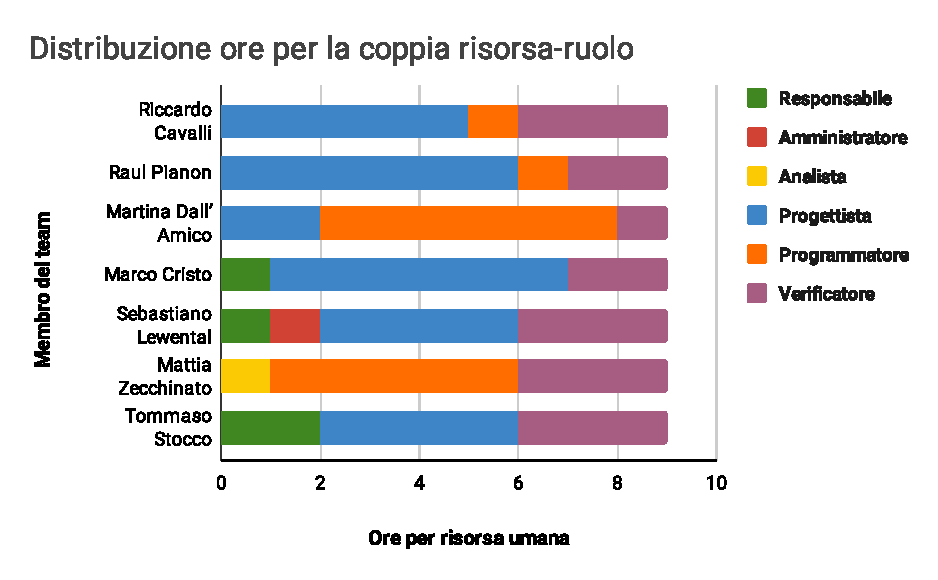
\includegraphics[width=0.90\textwidth]{assets/Consuntivo/Sprint-10/distribuzione_ore_risorsa_ruolo.pdf}
    \caption{Sprint 10 - Istogramma della distribuzione oraria per la coppia risorsa-ruolo}
  \end{figure}

  \begin{figure}[H]
    \centering
    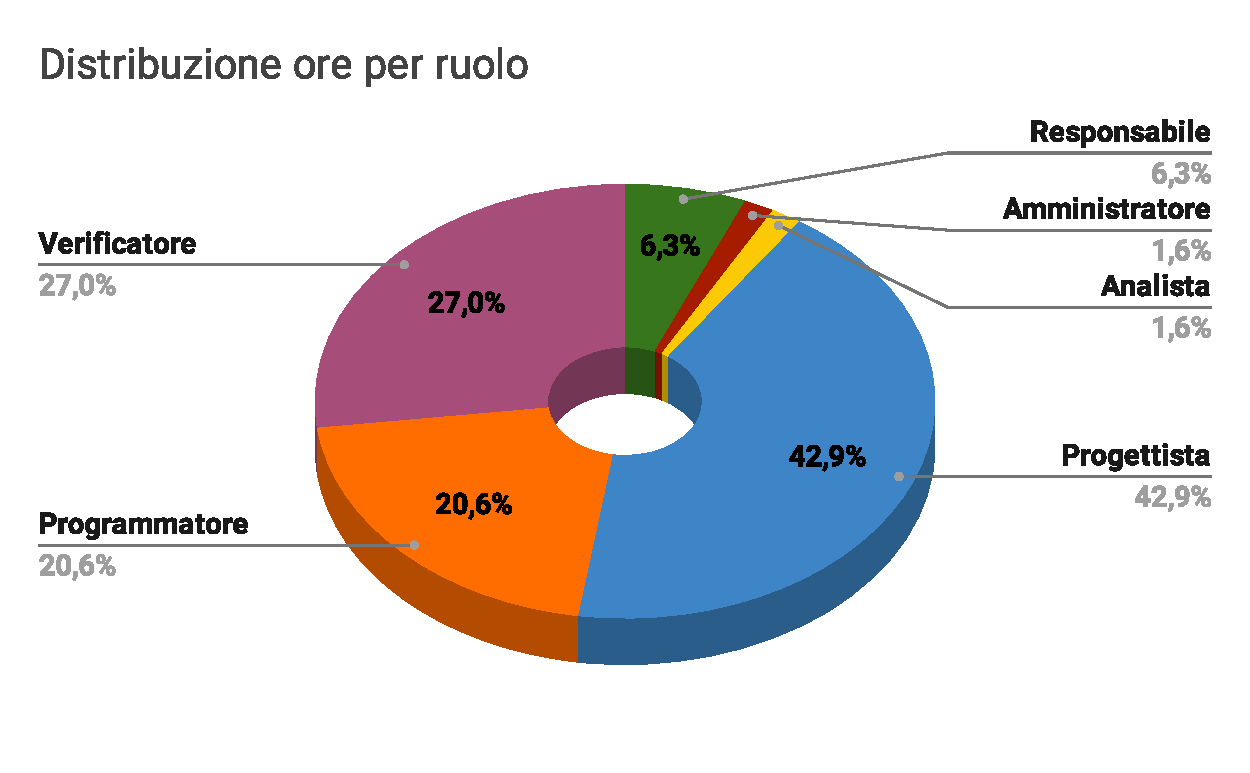
\includegraphics[width=0.90\textwidth]{assets/Consuntivo/Sprint-10/distribuzione_ore_ruolo.pdf}
    \caption{Sprint 10 - Areogramma della distribuzione oraria per ruolo}
  \end{figure}

  \begin{minipage}{\textwidth}
  Di seguito è riportato il consuntivo economico del decimo \glossario{sprint}:
  \begin{table}[H]
  \begin{adjustwidth}{-0.5cm}{-0.5cm}
    \centering
    \begin{tabular}{|P{2.9cm}|P{2.3cm}|P{2.5cm}|P{2.3cm}|>{\arraybackslash}P{2.5cm}|}
      \hline
      \multicolumn{5}{|c|}{\textbf{Consuntivo economico}} \\
      \hline
      \textbf{Ruolo} & \textbf{Ore per ruolo} & \textbf{Delta ore preventivo - consuntivo} & \textbf{Costo (in \texteuro)} & \textbf{Delta costo preventivo - consuntivo (in \texteuro)} \\
      \hline
      \Responsabile[U]{} & 4 & 0 & 120,00 & 0,00 \\ \hline
      \Amministratore[U]{} & 1 & 1 & 20,00 & 20,00 \\ \hline
      \Analista[U]{} & 1 & 0 & 25,00 & 0,00 \\ \hline
      \Progettista[U]{} & 27 & 3 & 675,00 & 75,00 \\ \hline
      \Programmatore[U]{} & 13 & -2 & 195,00 & -30,00 \\ \hline
      \Verificatore[U]{} & 17 & -1 & 255,00 & -15,00 \\ \hline
      \textbf{Totale} & \textbf{63} & 1 & \textbf{1.290,00} & 50,00 \\ \hline
      \textbf{Restante} & 219 & / & 4.420,00 & / \\ \hline
      \textbf{Sprint pregressi} & 364 & / & 7.310,00 & / \\ \hline
    \end{tabular}
    \caption{Sprint 10 - Consuntivo economico}
  \end{adjustwidth}
  \end{table}
  \end{minipage}

  \begin{figure}[H]
    \centering
    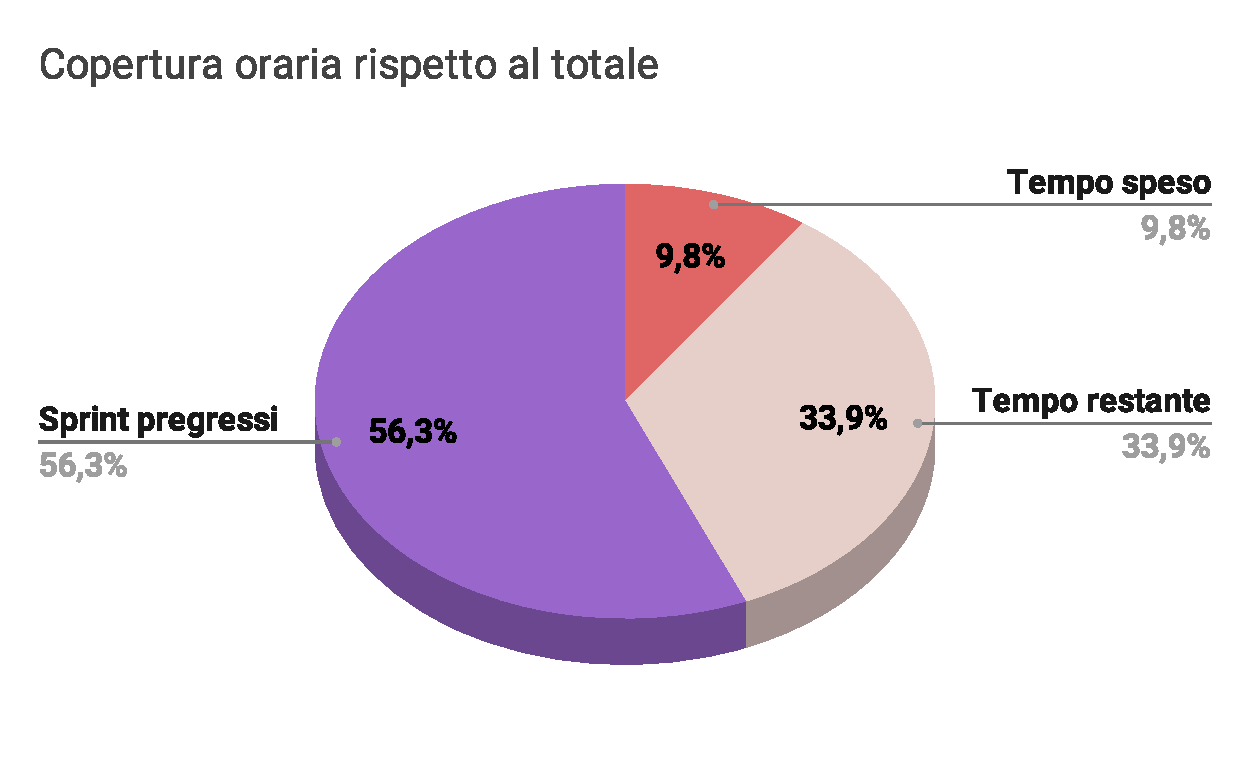
\includegraphics[width=0.90\textwidth]{assets/Consuntivo/Sprint-10/copertura_oraria.pdf}
    \caption{Sprint 10 - Areogramma del tempo speso (in ore) rispetto al totale}
  \end{figure}

  \begin{figure}[H]
    \centering
    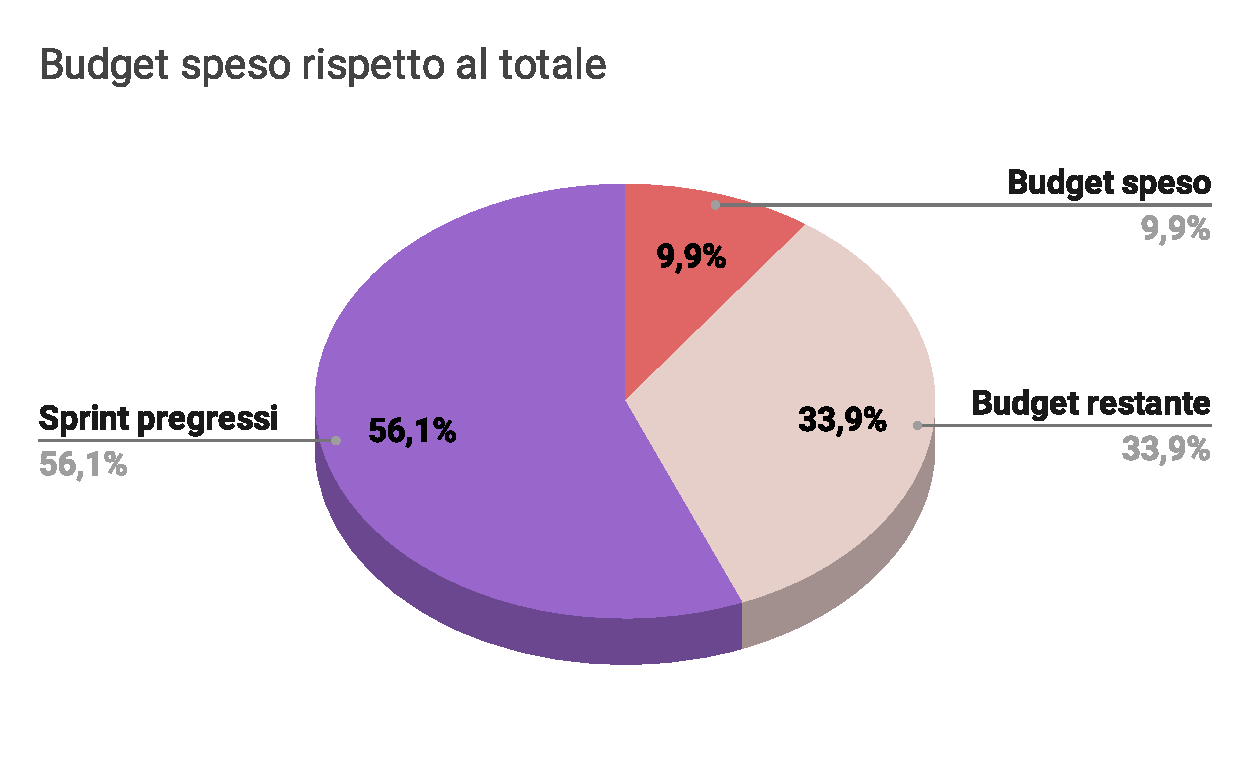
\includegraphics[width=0.90\textwidth]{assets/Consuntivo/Sprint-10/budget_speso.pdf}
    \caption{Sprint 10 - Areogramma del budget speso rispetto al totale}
  \end{figure}

  \begin{minipage}{\textwidth}
    Di seguito sono riportate le ore rimanenti per la coppia risorsa-ruolo:
    \begin{table}[H]
      \begin{tabularx}{\textwidth}{|c|*{6}{>{\centering}X|}c|}
        \hline
        \multicolumn{8}{|c|}{\textbf{Ore rimanenti per la coppia risorsa-ruolo}} \\
        \hline
        \textbf{Membro del team} & \textbf{Re} & \textbf{Am} & \textbf{An} & \textbf{Pt} & \textbf{Pr} & \textbf{Ve} & \textbf{Totale per persona} \\
        \hline
        Riccardo Cavalli & 0 & 1 & 3 & 7 & 9 & 6 & 26 \\
        \hline
        Raul Pianon & 2 & 1 & 1 & 13 & 9 & 4 & 30 \\
        \hline
        Martina Dall'Amico & 2 & 1 & 1 & 12 & 10 & 7 & 33 \\
        \hline
        Marco Cristo & 1 & 4 & 0 & 11 & 10 & 5 & 31 \\
        \hline
        Sebastiano Lewental & 2 & 3 & 1 & 7 & 11 & 8 & 32 \\
        \hline
        Mattia Zecchinato & 5 & 2 & 2 & 9 & 6 & 8 & 32 \\
        \hline
        Tommaso Stocco & 3 & 0 & 3 & 15 & 9 & 5 & 35 \\
        \hline
        \textbf{Totale ore per ruolo} & 15 & 12 & 11 & 74 & 64 & 43 & \textbf{219} \\
        \hline
      \end{tabularx}
      \caption{Sprint 10 - Ore rimanenti per la coppia risorsa-ruolo}
    \end{table}
  \end{minipage}

\subsubsection{Revisione delle attività}

Nell'arco del decimo \glossario{sprint}, il team ha svolto le seguenti attività:
\begin{itemize}
 \item Verifica e rilascio dei seguenti documenti:
  \begin{itemize}
    \item \NdP;
    \item \PdP;
    \item \AdR{} (post colloquio \RTB);
    \item \PdQ.
  \end{itemize}
  \item Correzioni alla documentazione post revisione \glossario{RTB};
  \item Stesura verbali interni;
  \item Aggiornamento dei grafici nel \PdQ;
  \item Miglioramento e formalizzazione delle convenzioni per lo stile di codifica;
  \item Progettazione architetturale \glossario{front-end};
  \item Progettazione logica \glossario{back-end};
  \item Modifica della struttura del front-end;
  \item Valutazione di possibili architetture per il back-end;
  \item Stesura di una relazione sulle architetture individuate;
  \item Progettazione di dettaglio front-end;
  \item Progettazione del database;
  \item Definizione di nuovi \glossario{dizionari dati};
  \item Selezione degli strumenti di test;
  \item Sperimentazione dei test di unità con pytest e Jest;
  \item Codifica e test di unità front-end;
  \item Configurazione di strumenti di formattazione e \glossario{linting} del codice;
  \item Stesura del documento \ST;
  \item Stesura del \MU\ (sezioni riguardanti la chat, la gestione dei dizionari e la configurazione delle impostazioni);
  \item Aggiornamento del file \textit{README} e dei requisiti di sistema;
  \item Utilizzo di \glossario{SonarLint} per il calcolo della complessità dei metodi.
\end{itemize}

\subsubsection{Retrospettiva}

\par Di seguito sono riportati i risultati del questionario di valutazione dello \glossario{sprint}:
\begin{itemize}
  \item Organizzazione dello sprint - Valutazione: 8;
  \item Conduzione dei meeting interni - Valutazione: 8.5;
  \item Impegno e partecipazione dei singoli membri - Valutazione: 7;
  \item Tutti i membri del team erano a conoscenza delle proprie mansioni;
  \item La numerosità delle riunioni è risultata adeguata per quasi tutti i membri del gruppo;
  \item Le riunioni sono state organizzate quasi sempre con il giusto preavviso;
  \item Il rapporto ore spese/ore produttive e la produttività generale sono migliorati rispetto agli sprint precedenti.
\end{itemize}

\vspace{0.5\baselineskip}
\par A seguire le \textbf{analisi a posteriori} del decimo \glossario{sprint}:
\begin{itemize}
  \item Il gruppo ha superato con successo la revisione \glossario{RTB}, dimostrando una solida comprensione degli obiettivi del capitolato e delle tecnologie necessarie per conseguirli;
  \item Durante la fase centrale dello sprint, il monitoraggio delle attività è stato meno costante rispetto al resto del periodo. Poiché il team ha deciso di tornare alla formula di sprint di due settimane, è necessario un controllo continuo da parte del responsabile;
  \item La progettazione del \glossario{back-end} ha comportato una fase iniziale di valutazione delle architetture potenziali. Questo ha causato un rallentamento nelle attività di progettazione e codifica;
  \item Il team di progettisti ha lavorato alla ristrutturazione del \glossario{front-end}, conseguendo una significativa riduzione della complessità dei metodi e delle funzioni;
  \item Il gruppo ha configurato strumenti per formattare automaticamente il codice prima di ogni commit. Questa configurazione riduce le problematiche legate al caricamento e all'estrazione del codice dal \glossario{repository} remoto;
  \item Inoltre, sono stati configurati strumenti di linting per eseguire un'analisi statica del codice prima di ogni commit;
  \item L'amministratore ha incontrato difficoltà nel reperire strumenti per il calcolo automatico delle metriche di qualità del codice. A partire dal prossimo sprint, verranno allocate più risorse per affrontare questa attività;
  \item Il team ha incrementato l'efficienza di merge delle pull request, stabilendo un ritmo soddisfacente per la verifica, approvazione e integrazione delle modifiche;
  \item Il gruppo ha configurato l'ambiente di test per il back-end e il front-end. In vista del prossimo sprint, l'obiettivo è definire un workflow su \glossario{GitHub} che garantisca la conformità del codice caricato nel repository agli standard previsti.
\end{itemize}

\subsubsection{Aggiornamento pianificazione e preventivo}
\par Il team ha definito un piano d'azione per migliorare l'organizzazione e la produttività del prossimo \glossario{sprint}:
\begin{itemize}
  \item Pianificare gli incontri con almeno un giorno di anticipo;
  \item Lavorare in team di due o più persone per le attività di progettazione, codifica e testing;
  \item Maggior focus e allocazione di risorse per la progettazione e codifica \glossario{back-end};
  \item Individuazione di strumenti per il calcolo automatico delle metriche di qualità del codice.
\end{itemize}

\paragraph*{Pianificazione futura:}
\par Nel corso dello \glossario{sprint}, il team si è concentrato sulla progettazione del \glossario{front-end}, che ha raggiunto un buon livello di dettaglio. Inoltre, il gruppo ha compiuto significativi progressi nella codifica del front-end. Per quanto riguarda il \glossario{back-end}, il team ha progettato il \glossario{database} e scelto il modello architetturale da seguire. Di conseguenza, il prossimo sprint sarà dedicato alla progettazione di dettaglio e alla codifica del back-end.

\par Durante lo sprint appena concluso, il gruppo ha definito ulteriori convenzioni per lo stile di codifica, che saranno formalizzate nelle \NdP\ nel prossimo sprint. Inoltre, verranno progettati i test di unità e saranno eseguiti test manuali utilizzando database locali e \glossario{dizionari dati} complessi.

\paragraph*{Preventivo "a finire" (\sezione{sec:stima_temporale}):}
\par Come illustrato nella \sezione{sec:preventivo-a-finire}, le ore riportate nel preventivo "a finire" sono equamente distribuite tra i membri del team. La maggior parte delle ore è assegnata ai ruoli di progettista, programmatore e verificatore; pertanto, il gruppo non ha ritenuto necessaria una ridistribuzione delle ore. Il team prevede di rispettare il budget preventivato e di completare il progetto entro la data di consegna prevista per metà settembre.

\paragraph*{Gestione dei rischi (\sezione{sec:analisi_rischi}):}
\par Durante il decimo \glossario{sprint}, i seguenti rischi sono stati gestiti con successo:
\begin{itemize}
  \item \textbf{RT3 - Malfunzionamenti software}: il gruppo ha riscontrato degli errori durante la costruzione delle immagini \glossario{Docker}. Inoltre, sono state eseguite attività di configurazione e refactoring che hanno generato malfunzionamenti software. Queste attività includono:
  \begin{itemize}
    \item Configurazione di strumenti per la formattazione e il \glossario{linting} del codice;
    \item Impostazione di software per la generazione automatica della documentazione;
    \item Creazione di funzioni componibili con \glossario{Vue.js};
    \item Configurazione degli strumenti di test.
  \end{itemize}
  Nonostante la complessità di alcuni errori, il team ha prontamente risolto i problemi attraverso l'apertura di ticket e discussioni nelle apposite sezioni di \glossario{GitHub}. Quando necessario, sono stati organizzati incontri specifici per la risoluzione tempestiva di bug e malfunzionamenti.
\end{itemize}
\subsection{Sprint 11: da 2024-08-05 a 2024-08-18}
\begin{minipage}{\textwidth}
Di seguito è riportata la distribuzione delle ore per ciascun membro del team, accumulate in totali per persona e per ruolo:
\begin{table}[H]
  \begin{tabularx}{\textwidth}{|c|*{6}{>{\centering}X|}c|}
    \hline
    \multicolumn{8}{|c|}{\textbf{Preventivo orario}} \\
    \hline
    \textbf{Membro del team} & \textbf{Re} & \textbf{Am} & \textbf{An} & \textbf{Pt} & \textbf{Pr} & \textbf{Ve} & \textbf{Totale per persona} \\
    \hline
    Riccardo Cavalli & 0 & 0 & 2 & 2 & 2 & 1 & 7 \\
    \hline
    Raul Pianon & 0 & 0 & 0 & 7 & 2 & 1 & 10 \\
    \hline
    Martina Dall'Amico & 0 & 0 & 0 & 6 & 3 & 1 & 10 \\
    \hline
    Marco Cristo & 0 & 2 & 0 & 4 & 4 & 0 & 10 \\
    \hline
    Sebastiano Lewental & 0 & 2 & 0 & 2 & 3 & 3 & 10 \\
    \hline
    Mattia Zecchinato & 3 & 0 & 0 & 3 & 1 & 3 & 10 \\
    \hline
    Tommaso Stocco & 1 & 0 & 0 & 6 & 2 & 1 & 10 \\
    \hline
    \textbf{Totale ore per ruolo} & 4 & 4 & 2 & 30 & 17 & 10 & \textbf{67} \\
    \hline
  \end{tabularx}
  \caption{Sprint 11 - Preventivo orario}
\end{table}
\end{minipage}

\begin{figure}[H]
  \centering
  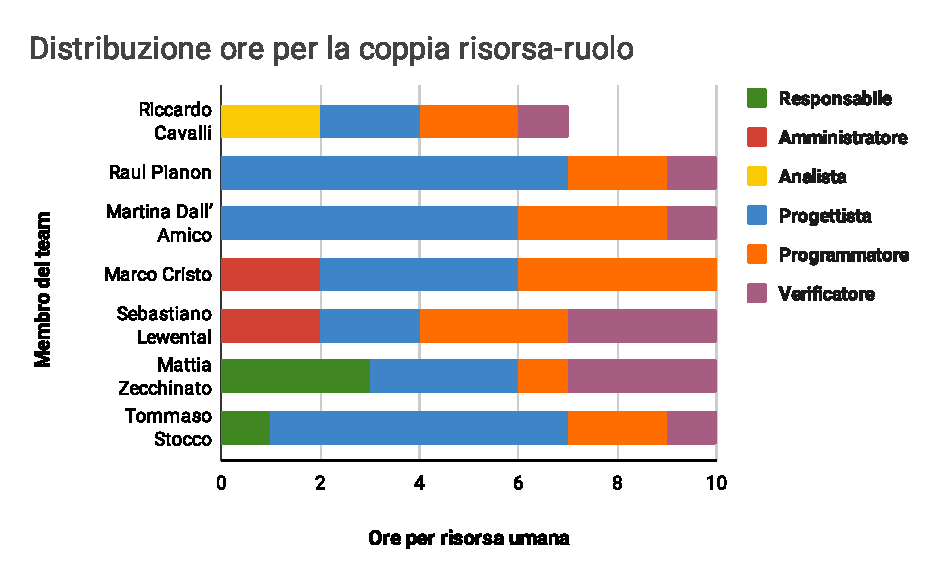
\includegraphics[width=0.90\textwidth]{assets/Preventivo/Sprint-11/distribuzione_ore_risorsa_ruolo.pdf}
  \caption{Sprint 11 - Istogramma della distribuzione oraria per la coppia risorsa-ruolo}
\end{figure}

\begin{figure}[H]
  \centering
  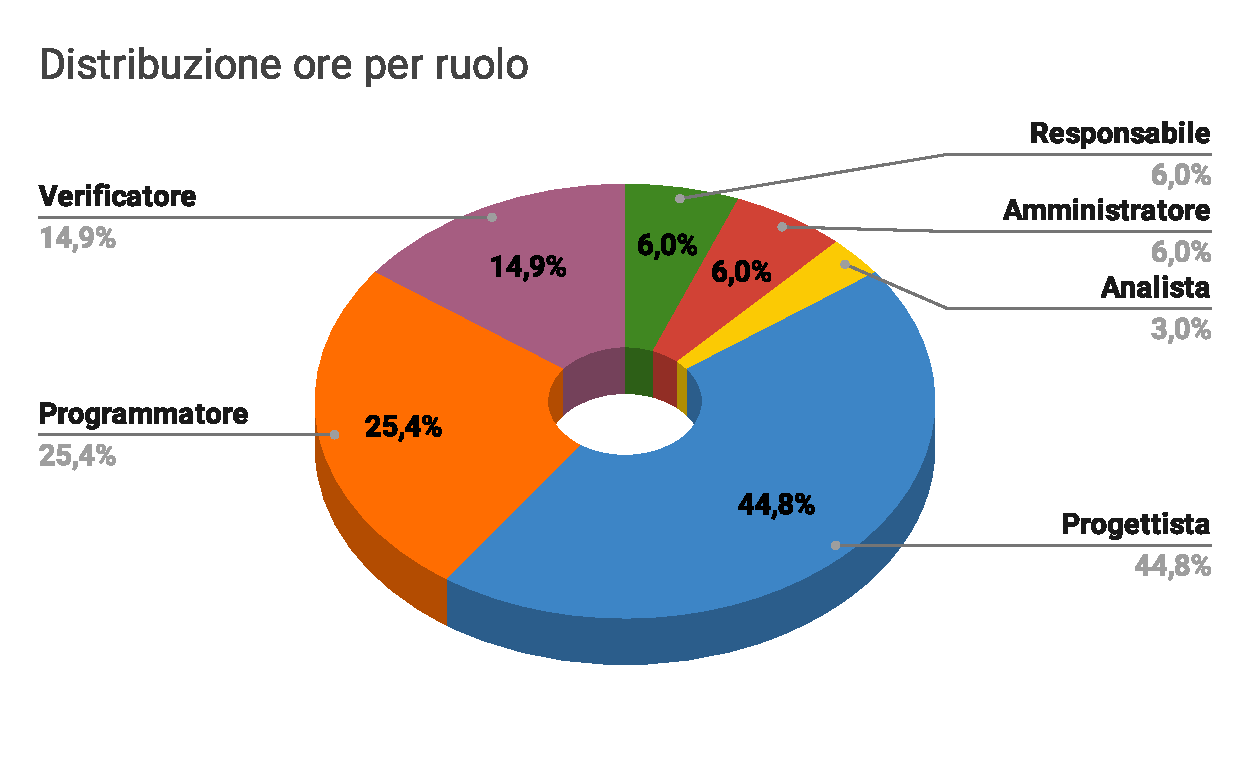
\includegraphics[width=0.90\textwidth]{assets/Preventivo/Sprint-11/distribuzione_ore_ruolo.pdf}
  \caption{Sprint 11 - Areogramma della distribuzione oraria per ruolo}
\end{figure}

\begin{minipage}{\textwidth}
Di seguito è riportato il preventivo economico dell'undicesimo \glossario{sprint}:
\begin{table}[H]
  \centering
  \begin{tabular}{|c|c|c|}
    \hline
    \multicolumn{3}{|c|}{\textbf{Preventivo economico}} \\
    \hline
    \textbf{Ruolo} & \textbf{Ore per ruolo} & \textbf{Costo (in \texteuro)} \\
    \hline
    \Responsabile[U]{} & 4 & 120,00 \\
    \hline
    \Amministratore[U]{} & 4 & 80,00 \\
    \hline
    \Analista[U]{} & 2 & 50,00 \\
    \hline
    \Progettista[U]{} & 30 & 750,00 \\
    \hline
    \Programmatore[U]{} & 17 & 255,00 \\
    \hline
    \Verificatore[U]{} & 10 & 150,00 \\
    \hline
    \textbf{Totale} & 67 & \textbf{1.405,00} \\
    \hline
  \end{tabular}
  \caption{Sprint 11 - Preventivo economico}
\end{table}
\end{minipage}

\subsection{Sprint 12: da 2024-08-19 a 2024-09-02}
\begin{minipage}{\textwidth}
Di seguito è riportata la distribuzione delle ore per ciascun membro del team, accumulate in totali per persona e per ruolo:
\begin{table}[H]
  \begin{tabularx}{\textwidth}{|c|*{6}{>{\centering}X|}c|}
    \hline
    \multicolumn{8}{|c|}{\textbf{Preventivo orario}} \\
    \hline
    \textbf{Membro del team} & \textbf{Re} & \textbf{Am} & \textbf{An} & \textbf{Pt} & \textbf{Pr} & \textbf{Ve} & \textbf{Totale per persona} \\
    \hline
    Riccardo Cavalli & 0 & 0 & 1 & 3 & 3 & 1 & 8 \\
    \hline
    Raul Pianon & 1 & 1 & 0 & 4 & 3 & 1 & 10 \\
    \hline
    Martina Dall'Amico & 1 & 0 & 1 & 4 & 3 & 2 & 11 \\
    \hline
    Marco Cristo & 1 & 1 & 0 & 3 & 3 & 1 & 9 \\
    \hline
    Sebastiano Lewental & 0 & 2 & 0 & 3 & 3 & 2 & 10 \\
    \hline
    Mattia Zecchinato & 2 & 0 & 2 & 2 & 2 & 2 & 10 \\
    \hline
    Tommaso Stocco & 0 & 0 & 2 & 4 & 4 & 2 & 12 \\
    \hline
    \textbf{Totale ore per ruolo} & 5 & 4 & 6 & 23 & 21 & 11 & \textbf{70} \\
    \hline
  \end{tabularx}
  \caption{Sprint 12 - Preventivo orario}
\end{table}
\end{minipage}

\begin{figure}[H]
  \centering
  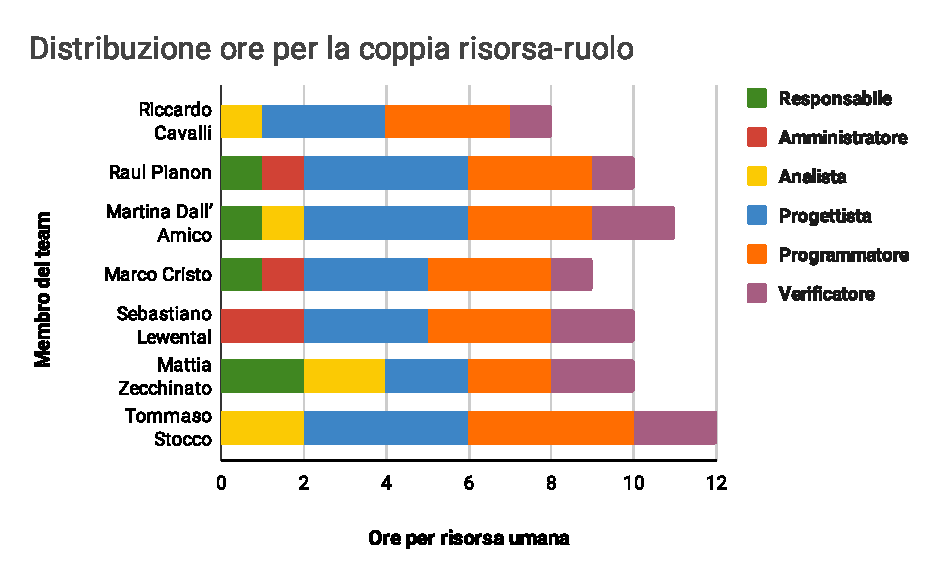
\includegraphics[width=0.90\textwidth]{assets/Preventivo/Sprint-12/distribuzione_ore_risorsa_ruolo.pdf}
  \caption{Sprint 12 - Istogramma della distribuzione oraria per la coppia risorsa-ruolo}
\end{figure}

\begin{figure}[H]
  \centering
  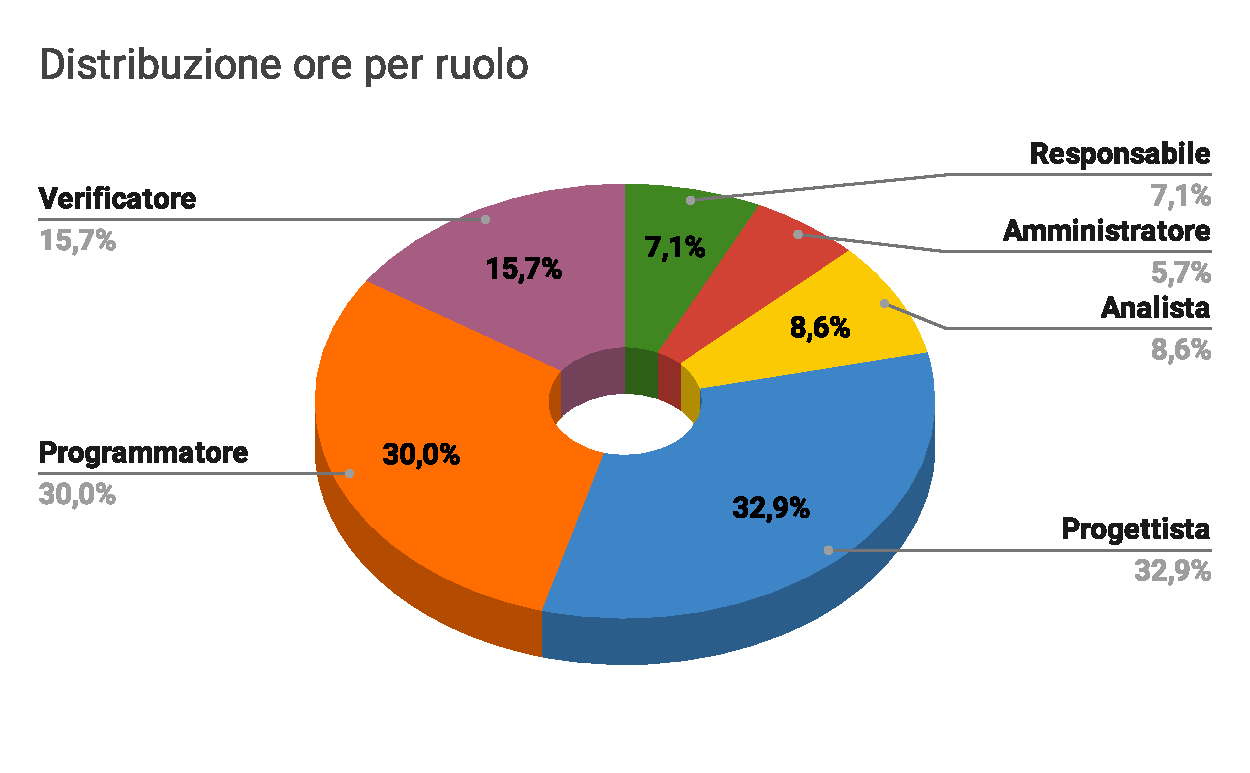
\includegraphics[width=0.90\textwidth]{assets/Preventivo/Sprint-12/distribuzione_ore_ruolo.pdf}
  \caption{Sprint 12 - Areogramma della distribuzione oraria per ruolo}
\end{figure}

\begin{minipage}{\textwidth}
Di seguito è riportato il preventivo economico del dodicesimo \glossario{sprint}:
\begin{table}[H]
  \centering
  \begin{tabular}{|c|c|c|}
    \hline
    \multicolumn{3}{|c|}{\textbf{Preventivo economico}} \\
    \hline
    \textbf{Ruolo} & \textbf{Ore per ruolo} & \textbf{Costo (in \texteuro)} \\
    \hline
    \Responsabile[U]{} & 5 & 150,00 \\
    \hline
    \Amministratore[U]{} & 4 & 80,00 \\
    \hline
    \Analista[U]{} & 6 & 150,00 \\
    \hline
    \Progettista[U]{} & 23 & 575,00 \\
    \hline
    \Programmatore[U]{} & 21 & 315,00 \\
    \hline
    \Verificatore[U]{} & 11 & 165,00 \\
    \hline
    \textbf{Totale} & 70 & \textbf{1.435,00} \\
    \hline
  \end{tabular}
  \caption{Sprint 12 - Preventivo economico}
\end{table}
\end{minipage}

